\documentclass[preprint,12pt]{elsarticle}

% International Journal of Plasticity (Elsevier), official elsarticle layout.
% Upload this file plus the figures/ folder to Overleaf, where elsarticle.cls
% ships with TeX Live. The article-class surrogate manuscript.tex builds the
% same content locally; body, bibliography and declarations are identical.

\journal{International Journal of Plasticity}

\usepackage[utf8]{inputenc}
\usepackage{amsmath}
\usepackage{graphicx}
\usepackage{booktabs}
\usepackage{caption}
\captionsetup{labelformat=empty, labelsep=none}
\setlength{\emergencystretch}{3em}

\begin{document}

\begin{frontmatter}

\title{Grain-boundary network percolation meets machine-learned grain-boundary energies: blind prediction of intergranular failure susceptibility}

\author[zl]{Han Wang\corref{cor1}}
\ead{wanghan2304@zhejianglab.org}
\cortext[cor1]{Corresponding author.}
\author[zj,zl]{Mengjia Chen}
\author[zz]{Mingxiang Liu}

\affiliation[zl]{organization={Zhejiang Lab},
  addressline={2880 Wenyi West Rd}, city={Hangzhou}, postcode={311121}, country={China}}
\affiliation[zj]{organization={School of Materials Science and Engineering, Zhejiang University},
  city={Hangzhou}, country={China}}
\affiliation[zz]{organization={Zhongyuan Critical Metals Laboratory, Zhengzhou University},
  city={Zhengzhou}, postcode={450001}, country={China}}

\begin{abstract}
Intergranular failure is a percolation event: susceptible boundaries must form a spanning path before cracking proceeds. We rank intergranular failure under a fixed equivalent-damage rule for Cu, Ni and Fe: machine-learned boundary energies decorate Voronoi microstructures with percolation descriptors, crystal-plasticity supplies labels, and grouped ablations, a twenty-microstructure blind test and an error-propagation audit quantify what the model knows. Topology alone blind-predicts percolation at AUC 0.774 (95\% CI 0.62--0.90); the full random forest (RF-TG) reaches 0.799 and the linear baseline (Lin-TG) 0.825 --- overlapping intervals: parity within present uncertainty; strain regression reaches \textit{R}$^{2}$ 0.26--0.38. A decoupled control removing $\gamma$ from the damage strength drops the energy-only channel to near-chance (CV AUC 0.584) while topology barely moves: part of the energy advantage is \textit{constructed} by the rule. An independent phase-field cross-check is directionally consistent with the ranking but bounds it, arresting 22--38\% of the rule-percolated cases rather than certifying the label. Perturbation is absorbed, not amplified: 7.0\% of flips lie below the label's cross-potential instability (10.8\%) and propagation gains remain below unity. Rankings hold under a fixed synthetic-label rule; marginal conformal coverage holds, conditional coverage remains open under the frozen protocol; closing it costs 2--4$\times$ per-metal calibration rows and $\sim$25\% wider intervals.
\end{abstract}

\begin{keyword}
grain boundary \sep percolation \sep crystal plasticity \sep intergranular failure \sep machine-learned interatomic potentials \sep conformal prediction
\end{keyword}

\end{frontmatter}

\section{Introduction}

Grain-boundary engineering (GBE) --- the design of boundary networks to control intergranular fracture [1] --- rests on a percolation idea [2]: microstructural failure along boundaries is not a single-boundary property but a connectivity property --- a connected path of susceptible boundaries must span the specimen before intergranular cracking proceeds systemically. This narrative is well established experimentally, notably in austenitic stainless steels where $\Sigma$3-boundary networks interrupt damage paths and improve resistance [3,4]. What the experimental programme has generally lacked is a predictive, quantitative counterpart: given a boundary-energy spectrum and a network graph, \textit{which} microstructure fails first, and how confidently?

Two mature computational ingredients now make such a model conceivable. First, machine-learned interatomic potentials (MLIPs) such as chgnet [5] and MACE-MP [6] --- products of the now-mature machine-learning approach to molecular and materials science [7] --- evaluate grain-boundary energies at DFT-like cost, and recent audits have begun quantifying their accuracy across hundreds of boundary configurations [8]. Second, graph representations of structure have become standard in materials property prediction (crystal graph convolutional neural networks [9]), and graph and percolation statistics of boundary networks are cheap to compute. What is missing --- the gap this paper occupies --- is the \textit{composition}: boundary energy $\times$ network topology $\rightarrow$ failure label $\rightarrow$ blind machine-learning test, with uncertainty quantification (UQ) and an error-propagation audit end to end. The nearest neighbours stop short: grain-level fatigue indicator GNNs treat boundaries as graph edges but target fatigue indicators rather than percolative failure [10]; MLIP boundary-energy evaluations stop at energy accuracy [8]; GBE percolation studies remain experimental [3]. We therefore also \textit{bound} the label rather than only report it: an independent phase-field fracture engine, given nothing but the same boundary-energy map, is directionally consistent with the ordering while showing that the rule is systematically more permissive.

We organise the gap as three research questions:

\begin{itemize}
\item \textbf{RQ1} --- To what extent do topological statistics of the non-twin boundary network (connectivity, winding thresholds, cluster statistics) determine intergranular failure susceptibility, relative to the boundary energies themselves?
\item \textbf{RQ2} --- Can a model driven by MLIP boundary energies and network-graph features blind-predict failure susceptibility for unseen microstructures (varying grain count, twin density, twin-length fraction), and where is the applicability-domain boundary?
\item \textbf{RQ3} --- How much does MLIP boundary-energy error propagate along ``energy $\rightarrow$ network features $\rightarrow$ failure prediction'' --- do topological features absorb or amplify atomic-level error?
\end{itemize}

The crystal-plasticity constitutive choice is phenomenological rather than mechanism-specific, justified by the ranking target: the label depends on the relative distribution of boundary-normal stress across the network, not on the absolute flow-stress level, and the ranking is shown to survive alternative damage laws (Sec. 2.7) and an independent elastic fracture engine (Sec. 2.8).

Our contributions are five-fold: (1) an \textit{audited} boundary-energy spectrum for three metals $\times$ three potentials with an explicit two-layer error structure (Sec. 2.1); (2) a microstructure library of 200 periodic Voronoi RVEs with energy-decorated percolation descriptors and 360 CPFEM-derived failure labels under a transparent equivalent-damage model (Secs. 2.2--2.3); (3) a leakage-controlled ablation and blind test with split-conformal UQ and a k-nearest-neighbour applicability domain (Secs. 2.4--2.5), together with a damage-law robustness audit that re-labels the same stress histories under alternative rules and quantifies the label's $\gamma$-coupling (Sec. 2.7); (4) an error-propagation audit whose perturbation source is the \textit{measured} inter-potential spread rather than an assumed noise model (Sec. 2.6); and (5) an independent phase-field fracture cross-check on a 46-microstructure subset, which provides a directional bound on the ordering and quantifies how much more permissive the equivalent-damage rule is than a fracture-mechanics criterion (Sec. 2.8).

\section{Results}

\subsection{The spectra have a two-layer error structure (Fig. 1)}

Across all three metals, potentials disagree in \textit{kind}, not only in degree. At coherent-twin-type boundaries (low-lying energy scale; literature 21--24 mJ m$^{-2}$ for Cu [11] and 41--90 for Ni [12,13]), the potentials underestimate and can change sign: Cu $\Sigma$3(111) computes as $-14.4$ (chgnet), +5.4, +7.8; Ni $\Sigma$3(111) as +12.7, +1.4, $-0.4$. At high-angle boundaries the magnitude is broadly right but the spread is quantitative and reaches up to 3$\times$: the two MACE sizes put Cu $\Sigma$3(112) at 559--579, inside the ab initio window (547--684 [13,14]), while chgnet overshoots at 1002; Ni is systematically high --- $\Sigma$5(310) at 2234--3840 against a 1218--1262 window [15,16]; and Fe $\Sigma$5(210) spans 771--2492 across potentials against 1090--2000 [15,17]. One cell is the opposite of scattered: Fe $\Sigma$3(112) returns 113.7/177.3/176.5 under the three potentials --- the tightest inter-potential spread in the library (1.6$\times$) --- yet all three sit below the ab initio window (340--510 [15]), agreeing with one another while sharing a common low bias: a construction-level offset rather than potential noise. Fig. 1 plots the full spectra; the twin-layer sign flips and the Fe consensus anchor are annotated.

\subsection{Network features carry a percolation signature --- and potential identity}

Pooling all 1800 (microstructure $\times$ metal $\times$ potential) rows, twin-length fraction correlates positively but modestly with the normalised winding threshold (Pearson \textit{r} = 0.17; per metal: Cu 0.23, Ni 0.25, Fe $-0.05$). Aggregating $\gamma$ features per microstructure --- removing the potential-level scatter --- raises the correlation to \textit{r} = 0.46, i.e. the organisational signal is real but is partly masked, not created, by potential-level variation. That variation is itself informative: for the \textit{same} microstructure, $\gamma_{\mathrm{perc}}$ under different potentials separates by a median factor 1.5$\times$ (max 3.4$\times$). The energy channel therefore carries a measurable fingerprint of which potential produced it --- the raw material for RQ3.

\subsection{Failure labels are distributed and only partially percolated (Fig. 2)}

Of 360 labels, 155 (43.1\%) percolate within $\varepsilon$ $\le$ 0.06; failure strains span 0.009--0.06 with median 0.036 and no pile-up at the first output step (v2 calibration succeeded). Percolation counts by metal: Cu 64, Ni 56, Fe 35 (censored fractions 47\%, 53\%, 71\%). At the moment of percolation the failed boundary length fraction has median 0.128 --- failure is a \textit{partial}-failure connectivity event (a winding path of damaged boundaries), not wholesale fracture, which is the physically right regime for a percolation label. Percolated strains separate visibly by potential within each metal (Fig. 2, left), confirming that the potential identity leaks into labels through $\sigma_{c}(\gamma)$ as designed --- and setting up the ablation.

\subsection{Ablation and blind test (Fig. 3, Table 1)}

Cross-validated (5$\times$4 grouped; mean $\pm$ fold-to-fold sd over the 20 folds, not a confidence interval): classification AUC rises T 0.799 $\pm$ 0.082 $\rightarrow$ G 0.816 $\pm$ 0.063 $\rightarrow$ TG 0.829 $\pm$ 0.064 (random forest); the linear baseline reaches 0.844 $\pm$ 0.055 on TG. Regression \textit{R}$^{2}$: T 0.247, G 0.403, TG 0.424 (RF; linear 0.263/0.362/0.295). Both channels carry signal, and the full feature set has the highest mean under grouped CV --- a point-estimate ordering, since the fold-to-fold sd's overlap.

On the twenty blind microstructures (180 rows; 100 non-censored), \textit{discrimination transfers}. The CV spread and the blind bootstrap CI are different quantities --- fold-to-fold variability of the fitting procedure versus sampling uncertainty over blind groups --- and are not directly compared. Percolation AUC = 0.799 (TG-RF, 95\% group-bootstrap CI 0.66--0.91) and 0.825 (TG-Lin, 0.71--0.92), against 0.774 (T-RF) and 0.767 (G-RF) --- every interval lies well above the 0.5 chance line; TG has the highest point estimate, but its group-bootstrap interval overlaps those of T and G, so the blind set does not resolve a ranking among feature sets. T and G trade places (0.774 vs 0.767) far inside those same overlapping intervals, so the two single channels are indistinguishable on the blind set. The original eight-microstructure point estimate (AUC 0.851 TG-RF; retained as a grey cross in Fig. 3) sits inside its own group-bootstrap interval (0.70--0.97) and inside the twenty-group interval: with only eight groups the point estimate was noisier than it looked, in the optimistic direction here. \textit{Magnitude also transfers once the blind set is large enough to measure it}: $\varepsilon_{\mathrm{fail}}$ regression gives \textit{R}$^{2}$ = 0.26--0.38 across models (G-RF 0.377, CI 0.09--0.59, and G-Lin 0.365, CI 0.09--0.54 --- the two G-feature intervals exclude zero, while the T- and TG-intervals touch it at the lower edge, e.g.\ TG-RF 0.299, CI $-0.07$--0.56), with MAE 0.0084--0.0092 strain units. The forest-versus-linear asymmetry seen on eight groups (forest apparently worse) does not survive the larger sample: the two models' intervals overlap throughout --- the honest reading is \textit{parity within present uncertainty}, not a ranking. On the twelve purely added microstructures alone (ext12 subset, coloured separately in the Fig. 3 scatter), the full model reaches AUC 0.770 (0.57--0.94) and \textit{R}$^{2}$ 0.44 (point estimate; group-bootstrap CI $-0.12$--0.74 touches zero at twelve groups) --- a genuine extrapolation set the frozen model never saw during any stage of fitting. This is the substantive RQ2 answer: the \textit{verdict} (does this microstructure percolate within 6\% strain?) blind-predicts at AUC $\approx$ 0.80 (CI excluding chance), the failure strain is recoverable at \textit{R}$^{2}$ $\approx$ 0.3 but its interval still touches zero --- both numbers now carry quantified uncertainty rather than single-group point estimates.

\subsection{Marginal coverage holds, conditional coverage remains open; the domain flag fires rarely (Fig. 4)}

Regression split-conformal 90\% intervals achieve blind coverage 0.86--0.99 across all six model/feature-set combinations on the twenty-microstructure set (TG-RF: 0.86, CI 0.74--0.96, at half-width 0.017 strain; TG-Lin: 0.99, 0.97--1.00, at 0.025 --- mildly conservative, as expected from a 36-row calibration set) --- consistent with the nominal 0.90; the calibration set's composition is unchanged by the blind-set extension. This is \textit{marginal} coverage pooled over metals and potentials; conditional coverage is not established. Split by metal, TG-RF gives 0.74 (Cu, $n$ = 43; 95\% Wilson interval 0.60--0.85, excluding the 0.90 nominal), 0.92 (Ni, $n$ = 39; 0.80--0.97) and 1.00 (Fe, $n$ = 18; 0.82--1.00) --- the linear baseline gives 0.98--1.00 --- so with 18--43 rows per metal the estimates are coarse, but the spread (Cu under-coverage under the forest, Fe over-coverage) is exactly why conditional coverage is flagged as open rather than claimed; the calibration set itself is metal-balanced (12 non-censored rows per metal), so the Cu shortfall is a genuine distribution question, not a calibration-composition artefact. An exploratory per-metal (Mondrian) recalibration does not repair the spread: with 12 calibration rows per metal the within-metal 90\% quantile is the maximum residual, so for TG-RF Cu barely moves (0.74 $\rightarrow$ 0.74) while Fe drops (1.00 $\rightarrow$ 0.61) and pooled coverage falls (0.86 $\rightarrow$ 0.80) --- metal stratification cannot remove the group-level shift between calibration and blind microstructures, so the binding constraint is per-metal calibration sample size, not the conformal variant (\texttt{results/e4c\_mondrian.csv}). To size that constraint, an expanded-calibration sensitivity run (\texttt{results/e4d\_cal\_sensitivity.csv}) augments the frozen 36-row pool with five-fold out-of-fold residuals from the 24 training groups (36 $\rightarrow$ 115 non-censored rows; per metal 12 $\rightarrow$ 48/41/26 for Cu/Ni/Fe). Models, split and blind set are untouched (these residuals never enter the frozen protocol; they exist only to size the calibration-sample constraint). Pooled over metals the extra rows change nothing --- TG-RF blind coverage stays 0.86 and Cu stays 0.74 --- confirming again that the Cu shortfall is a calibration-versus-blind distribution question rather than a pooled-sample-size artefact.

The per-metal 90\% quantile, however, is no longer the within-metal maximum: Mondrian coverage rises from 0.80 to 0.94 (95\% group-bootstrap CI 0.87--0.99), Cu recovering 0.74 $\rightarrow$ 0.91 and Fe 0.61 $\rightarrow$ 1.00, at a half-width cost of 0.017 $\rightarrow$ 0.021 strain (about a quarter wider). The linear baseline, in turn, sheds its mild conservatism once pooled over the expanded set (coverage 0.99 $\rightarrow$ 0.95 at half-width 0.025 $\rightarrow$ 0.021). The conditional-coverage gap is thus quantitatively closeable --- at roughly two to four times the per-metal calibration rows and about a quarter more interval width --- so the binding constraint is per-metal calibration sample size, a resource limit of the frozen protocol rather than a defect of split conformal. Because the added residuals are out-of-fold predictions on the training groups rather than an independent holdout, we report this as sensitivity analysis only, and the frozen-protocol numbers above remain the ones claimed. Folding them into the frozen protocol would compromise the blind-set purity that the protocol was designed to protect. The applicability domain ($\tau$ = 3.53) flags 6 of 180 blind rows as OOD (three in each of the original and added subsets); the flagged rows span all three potentials' regimes rather than one corner of feature space. Residuals do not blow up with $d_5$ in the blind set (Fig. 4, the original eight microstructures at full row resolution; the extended set is not re-plotted against $d_5$ --- per-row $d_5$ and domain flags live in \texttt{results/e4b\_prediction\_audit.csv}, and the two OOD rows among the 100 regression rows are marked in Fig. 3) --- with six OOD rows we read the flag as a \textit{guard rail} whose false-negative rate cannot yet be estimated, not as a proven residual predictor.

\subsection{Error propagation: absorbed within the pipeline, not amplified (Fig. 5)}

Perturbing every edge to a different potential's pool ($p$ = 1) moves the $\gamma$ features by median relative 18\% (mean $\gamma$), 24\% ($\gamma$ std), 19\%/15\% ($\gamma_{\mathrm{perc}}$ absolute/relative), 11\% (cluster AUC) and 3\% (failed fraction at mean) --- while all topology features move by exactly 0, and both the $p$ = 0 control and the \textbf{T}-only model show machine-zero drift throughout (self-checks pass).

At the prediction layer, the full model's binary verdict flips on 7.0\% of rows under full perturbation (4.8\%, 6.6\%, 6.9\% at $p$ = 0.25/0.5/0.75) --- \textit{below} the label's own cross-potential instability (13/120 = 10.8\% of censoring verdicts change when the label itself is regenerated under another potential). The predictor is thus more stable than its supervision. Regression predictions move by median $|\Delta\hat{\varepsilon}|$ = 0.0030 at $p$ = 1 --- about one third of the primary blind MAE (0.0084--0.0092; the original eight-group audit MAE is slightly larger, 0.0095--0.0114, computed row-wise from \texttt{results/prediction\_audit.csv}) --- and the propagation gain decays monotonically with $p$: $G$ = 0.76, 0.49, 0.42, 0.39 (all $<$ 1). The prediction layer \textit{compresses} relative input error; the topology-only channel admits none. RQ3's answer: within this pipeline, atomic-level energy error is absorbed at every stage it passes through, and the features that never see atoms are immune by construction.

\subsection{Label robustness under alternative damage laws (E6)}

The labels of Sec. 2.3 rest on one equivalent-damage rule; two re-labelling checks ask how much of the paper's conclusions ride on that choice. Both reuse the same 360 CPFEM stress histories, so no new simulation is involved. (The blind figures in this section are quoted on the original eight-group \textit{audit} set --- the re-labellings predate the Sec. 4.4 extension, so they are compared against the 0.851 baseline of that set rather than the twenty-group primary value; they are deliberately not re-benchmarked on the extended set.) For reference, the same TG-RF model scores 0.799 (0.66--0.91) on the twenty-group primary set; the eight-group values here are used only for like-for-like comparison with the pre-extension audits.

\textbf{Alternative coupled laws.} Re-labelling under linear accumulation ($m$ = 1), Griffith-like weaker coupling ($p$ = 0.5) and linear stronger coupling ($p$ = 1.0) uses a single per-metal gain on $\sigma_{c}$ (0.22--3.65, solved by log-bisection) so that every variant reproduces the baseline per-metal percolation counts (Cu 64 / Ni 56 / Fe 35) --- count matching is a diagnostic normalisation that isolates the \textit{shape} of the law from a trivial strength scale, never tuned against predictive performance --- and first-step pile-up stays at 0\% throughout. Under each variant the models are retrained from scratch with identical hyperparameters, seeds and group splits, so the comparison asks whether the conclusions survive a changed label rather than whether a fixed predictor does. Verdicts agree with the baseline on 97.2--100\% of rows; for $m$ = 1 the agreement is exactly 1.000 with all AUCs identical, because $m$ enters only as the stress-ratio exponent of the damage-accumulation rate ($D \propto \int (\sigma_{n}/\sigma_{c})^{m} dt$) --- halving it shifts damage timing without changing the realised connectivity pattern --- while $\varepsilon_{\mathrm{fail}}$ ordering is preserved throughout (Spearman $\rho$ 0.976--0.991). The ML conclusions hold: grouped CV AUC (TG-RF) 0.819--0.829 versus 0.829 baseline, blind AUC 0.827--0.855 versus 0.851, with the grouped-CV T $<$ G $<$ TG ablation order unchanged and the full model still best blind.

\textbf{Decoupled control ($\gamma$ removed from the strength).} With $\sigma_{c}$ constant per metal and percolation counts approximately re-matched (63/57/36 --- a constant per-metal strength cannot hit the baseline counts exactly), labels agree with the baseline on only 64.7\% of rows and the $\varepsilon_{\mathrm{fail}}$ ranking collapses to $\rho$ = 0.119 --- a direct measure of how much of the label is a function of $\gamma$. The G-only channel then loses most of its signal (grouped CV AUC 0.816 $\rightarrow$ 0.584; blind 0.807 $\rightarrow$ 0.542, i.e.\ chance) while T-only barely moves \textit{in grouped CV} (0.799 $\rightarrow$ 0.787); even the full-feature blind AUC falls from 0.851 to 0.663. On the 72-row blind audit set every decoupled random-forest channel drops relative to the baseline (T 0.823 $\rightarrow$ 0.639, G 0.807 $\rightarrow$ 0.542, TG 0.851 $\rightarrow$ 0.663), so the blind audit values are read ordinally --- G $<$ T $<$ TG, the CV ordering preserved --- while the level comparison behind ``G to chance, T stable'' rests on grouped CV; the residual CV TG $>$ T gap (0.810 vs 0.787) is within fold-to-fold sd and is not interpreted as signal. The standalone energy-channel advantage is thus largely \textit{constructed} by the $\sigma_{c}(\gamma)$ coupling --- quantifying the RQ1 caveat of Sec. 3 --- whereas the coupling-free topology channel is unchanged and remains the lower-bound estimate of the topological share.

\textbf{Twin-fraction proxy (a diagnostic under this rule, not an experimental GBE claim).} Spearman correlation of twin-length fraction with the percolation verdict is $+$0.326 pooled ($p$ $<$ 10$^{-9}$) but splits by metal: Fe is $-$0.303 ($p$ = 8 $\times$ 10$^{-4}$), consistent with $\Sigma$3 networks interrupting damage paths [3], while Cu ($+$0.658) and Ni ($+$0.587) are opposite to the classical narrative. Two features of the label generator account for the signs. The rule inverts physical intuition by construction: $\sigma_{c} \propto (\gamma + \gamma_0)^{p}$ makes \textit{low}-$\gamma$ boundaries the \textit{weak} ones --- a deliberate simplification of the label generator --- so the Cu/Ni positive correlation follows directly from the rule's energy channel (more twins $\rightarrow$ more low-$\gamma$ $\Sigma$3 edges $\rightarrow$ more low-$\sigma_{c}$ edges $\rightarrow$ easier percolation). Fe, with the lowest percolation rate of the three metals (35/120, 71\% censored), is consistent with a topology-dominated regime in which twin boundaries mainly \textit{segment} the network rather than supply weak links --- and a targeted probe confirms the negative sign does not come from the Fe anchor: raising $\gamma_0$(Fe) from 0 to the Cu/Ni values (22, 70) and re-running the full damage integration (re-sampled $\tilde{\gamma}$, re-calibrated $k$, percolation counts matched to 35 as in the E6 protocol) keeps $\rho$ negative throughout ($-0.303$, $-0.303$, $-0.299$ for $\gamma_0$ = 0, 22, 70), and without count matching the Fe counts shift $35 \rightarrow 28 \rightarrow 10$ while $\rho$ stays negative ($-0.303$, $-0.351$, $-0.253$); the $\gamma_0$ = 0 run reproduces the published labels row by row, and Cu/Ni are untouched by construction (\texttt{results/e6\_fe\_gamma0\_probe.csv}). This correlation is reported as a \textit{diagnostic} of how the fixed equivalent-damage rule maps network structure onto failure --- it is not evidence for or against classical GBE, and the metal dependence of the sign is precisely why every claim in this paper is framed as \textit{relative susceptibility rankings under a fixed rule} rather than absolute GBE expectations.

\subsection{An independent fracture engine recovers the ordering only partially (E7)}

The labels of Sec. 2.3 rest on a strength rule, and the re-labelling audits of Sec. 2.7 cannot test whether their \textit{ordering} survives a different failure physics, because every variant reuses the same CPFEM histories and the same connectivity criterion. We therefore re-solved the same microstructures with an independent engine: a two-dimensional plane-stress phase-field fracture model --- an AT2 functional with an irreversibility history field, periodic boundaries and staggered displacement--damage solves, written from scratch for this audit --- which shares only the boundary-energy map with the label pipeline. Its boundary fracture energy follows the same $\gamma \mapsto (\gamma+\gamma_0)^{p}$ form, normalised to 1 J m$^{-2}$ at the pool median, with a 100 J m$^{-2}$ grain interior that confines cracking to boundaries; the criterion, however, is energetic crack propagation rather than a stress-overload integral, and neither CPFEM nor a per-edge damage variable enters. Runs are loaded identically ($\varepsilon_{xx}$ to 0.06 in steps of 0.001, lateral $\varepsilon_{yy}$ iterated to zero mean $\sigma_{yy}$) and scored at the strain where the damage band winds across the periodic cell --- the same connectivity event as the label's winding test, and the only quantity the two engines share by construction. The subset is every microstructure whose labels percolate under all three potentials (Cu 20, Ni 18, Fe 8 --- Fe has exactly eight such cases), giving 138 runs.

The comparison is deliberately asymmetric in one respect. The label was constructed to percolate on this subset, whereas the phase-field engine percolates in only 62--78\% of the runs (Cu 37/60, Ni 42/54, Fe 15/24): an elastic engine carries more strain before a crack grows than a plasticity-mediated microstructure does, and absolute strains differ accordingly (label 0.009--0.057, phase-field 0.026--0.056). Ranking, not level, is therefore what the comparison can carry. With resolved cases ordered by strain and arrested cases ranked slowest, Spearman $\rho$ is positive in all nine (metal, potential) cells and spans 0.12--0.36 (median 0.23); pooling potentials within a metal gives 0.15, 0.14 and 0.19 for Cu, Ni and Fe (microstructure-cluster bootstrap intervals include zero), and a metal-centred pooled estimate over all 138 runs gives $\rho$ = 0.145 ($p$ = 0.09). Restricted to resolved cases only, Cu and Ni stay positive (0.15--0.35) while Fe turns negative ($-0.16$ to $-0.29$).

Two readings follow, and neither is a validation. First, the sign is consistent: an engine that knows nothing about the damage law still orders the microstructures in the same general direction, which is the most an external check can establish for a synthetic label, and the weak magnitude is consistent with the two engines answering different questions (an overload integral lets any sufficiently stressed boundary fail eventually, whereas a crack must actually propagate). Second, the verdicts disagree often enough to matter: the equivalent-damage rule is systematically \textit{more permissive} than a fracture-mechanics criterion, arresting in 22--38\% of the cases it labels as percolated. The cross-check therefore bounds the label rather than certifying it --- it is a relative-susceptibility ranking whose direction a fracture engine corroborates, not a failure simulation --- and the Fe sign reversal under the strict comparison mirrors the topology-dominated behaviour already reported for Fe in the twin-fraction proxy (Sec. 2.7).

\section{Discussion}

\textbf{RQ1 --- topology versus energy.} Topology alone reaches AUC 0.799 / \textit{R}$^{2}$ 0.247, so a substantial, coupling-free share of failure susceptibility lives in the graph; energy features add on top (TG $>$ G in both targets), and energy's larger regression increment (0.247 $\rightarrow$ 0.403) must be read with one honest caveat: the labels themselves are generated through $\sigma_{c}(\gamma)$ from the same E1 pools, so part of G's advantage is constructed, not discovered --- and the decoupled-label control (Sec. 2.7) puts numbers on it: removing $\gamma$ from the damage strength at approximately matched percolation flips 35\% of verdicts, collapses the $\varepsilon_{\mathrm{fail}}$ ranking to $\rho$ = 0.119, and drops the G-only channel to CV AUC 0.584 while T-only barely moves in grouped CV (0.799 $\rightarrow$ 0.787). T's performance is unaffected by that coupling and therefore stands as a \textit{lower bound} on the topological share; TG's gain over G is the clean evidence that topology contributes beyond energy --- the paper's joint-determination claim, with the two contributions disentangled rather than asserted.

\textbf{RQ2 --- blind generalisation and its boundary.} Discrimination survives the shift to unseen microstructures (AUC 0.799, group-bootstrap CI 0.66--0.91 across twenty blind groups, well clear of chance), and magnitude regression is recoverable but less certain (\textit{R}$^{2}$ 0.26--0.38; the full model's interval $-0.07$--0.56 touches zero). Three readings follow from the enlarged blind set: first, eight groups gave two noisy point estimates in opposite directions --- 0.851 AUC was optimistic, 0.078 \textit{R}$^{2}$ pessimistic, both inside the twenty-group intervals --- which is the statistical argument for reporting groups-bootstrap intervals rather than single-split values; second, the linear baseline and the forest are at parity within present uncertainty on both targets, so the response looks close to low-dimensional/monotone rather than forest-dominated; third, the conformal layer is not decoration --- intervals held nominal coverage (0.86--0.99) across the extended blind set exactly where point predictions carry wide intervals. The domain flag (6/180) is cheap and fires rarely at this sampling density; at larger scales its precision should be re-evaluated rather than assumed.

\textbf{RQ3 --- the propagation audit.} Using measured inter-potential spread as the perturbation source avoids inventing a noise model, and the exact replay of the E2 random stream makes the baseline reproducible to rounding. Two structural results dominate: topological features cannot carry atomic error (zero by construction, verified to machine precision), and the model layer absorbs the remainder ($G$ $<$ 1 at every $p$, flips below the label's own instability). The audit is within-pipeline --- perturbed features are scored against labels generated from unperturbed energies --- so it measures \textit{sensitivity of the trained predictor}, not end-to-end label regeneration; the latter is the natural extension and would likely widen the drift, though the label-side anchor (10.8\%) already brackets it.

\textbf{2D versus 3D percolation.} $\gamma_{\mathrm{perc}}$ is a winding threshold defined on a periodic two-dimensional cell, and percolation thresholds and critical exponents belong to dimensionality-dependent universality classes [2] --- the two-dimensional bond and site problems differ from their three-dimensional counterparts both in threshold values and in exponents, and so does the geometry of the spanning set. Two consequences follow for the transferability of $\gamma_{\mathrm{perc}}$. The \textit{form} of the descriptor carries over: the maximin cycle bottleneck is the energy-ordered connectivity statistic of a grain-boundary graph irrespective of embedding dimension, and a 3D network admits the same computation with wrapping in any of three directions. The \textit{calibration} does not: the numerical threshold, the winding criterion adopted here and the percolation verdict itself are established in the 2D columnar universality class and would have to be re-established in 3D, where the spanning geometry and critical scale differ [2]. Our columnar, 2D-periodic RVEs realise exactly the geometry in which $\gamma_{\mathrm{perc}}$ is defined, which is consistent with the framing used throughout: every reported number is a relative ranking under a fixed 2D rule, not a portable threshold: a $\gamma_{\mathrm{perc}}$ value reported here should not be compared across studies that define the winding threshold in 3D.

\textbf{Relation to prior work.} Where FIP-GNN maps boundary graphs to fatigue indicators [10] and MLIP audits map potentials to energies [8], we compose spectrum $\rightarrow$ graph $\rightarrow$ label $\rightarrow$ blind test $\rightarrow$ propagation audit. Machine-learned prediction of per-boundary damage susceptibility [21] addresses the same physical quantity one step earlier in the chain, at the level of individual boundaries; we lift that target to network-level percolation and test the resulting predictor on unseen microstructures. MLIP error propagation into continuum-scale predictions poses the same question one level downstream; here the propagated quantity is a \textit{feature within a learned predictor} rather than a downstream continuum field, closing the loop between the two narratives. On the fracture side, recent extended Rice--Thomson analyses resolve grain-boundary fracture criteria atomistically [18], hydrogen-assisted intergranular cracking is the canonical chemical route to intergranular failure [19], and MLIPs now target hydrogen-embrittlement mechanisms [20], but neither line --- nor the MLIP audits [8], the FIP-GNN [10] or the per-boundary damage predictor [21] --- composes energy spectrum, network topology and a validated failure label into a single blind-tested predictor; that composition is what this paper supplies, with UQ and an error-propagation audit attached.

\textbf{Limitations.} (i) Labels come from one equivalent-damage model, calibrated ($\kappa$, $p$, $\gamma_0$) rather than derived; claims are about \textit{relative susceptibility rankings under a fixed rule} --- the same protocol applied to any candidate microstructure --- not absolute failure strains. Sec. 2.7 re-labels the same stress histories under alternative $m$/$p$ laws and shows the rankings and ablation conclusions stable, and quantifies the $\gamma$-coupling via the decoupled control; Sec. 2.8 re-solves a 46-microstructure subset with an independent phase-field fracture engine, which reproduces the ordering direction but only weakly (median $\rho$ 0.23 across nine cells, none individually significant) and arrests in 22--38\% of the cases the rule labels as percolated, so the cross-check bounds the label rather than validating it, and no experimental cross-validation exists. The label is therefore a controlled synthetic target, not a validated GBE predictor: the Cu/Ni sign reversal in the twin-fraction proxy (Sec. 2.7) shows that the fixed rule does not reproduce classical GBE trends for all metals --- it is a property of the equivalent-damage rule, not evidence against classical GBE --- and it is precisely why all claims are framed as relative rankings under this rule and about the ML/UQ pipeline, not about absolute GBE physics; the paper is accordingly positioned as a methodological pipeline study rather than a physical-mechanism paper. (ii) RVEs are 2D-periodic and columnar, downsampled 4$\times$; periodicity removes free-surface effects but 3D crack-front topology is absent. (iii) Microstructures are synthetic Voronoi statistics rather than reconstructed EBSD. (iv) Blind scale is twenty microstructures (180 rows, 100 non-censored for regression), which still leaves wide intervals --- roughly $\pm$0.10--0.14 on AUC and $\pm$0.22--0.32 on \textit{R}$^{2}$ --- and conformal quantiles rest on 36 calibration rows whose composition (the original eight calibration groups) was not enlarged along with the test set; marginal coverage is established, conditional coverage remains open (Sec. 2.5, where an expanded-calibration sensitivity run quantifies the improvement space --- per-metal Mondrian coverage 0.80 $\rightarrow$ 0.94 at intervals a quarter wider --- without altering the frozen protocol); the out-of-fold residuals may be optimistically narrow relative to a genuinely independent calibration pool, so the 0.94 figure should be read as an upper bound on the achievable Mondrian coverage. (v) Literature anchors used to contextualise the spectra are cross-method windows (experimental, empirical-potential and ab initio values per cell), verified against the cited sources but still compilations spanning different methods; only three potentials sample the MLIP error distribution.

\subsection{Conclusions}

\begin{enumerate}
\item \textbf{Joint determination.} Intergranular failure susceptibility under a fixed damage rule is carried by both boundary-network topology and the boundary-energy spectrum; each channel predicts out of sample, and the full feature set is best under grouped cross-validation (AUC 0.829, \textit{R}$^{2}$ 0.424). The energy channel's larger increment is partly constructed by the $\gamma$-dependent label rule rather than discovered --- the topology-only result is immune to that coupling and therefore a lower bound on the topological share, while TG over G is the clean evidence that topology contributes beyond energy.
\item \textbf{Blind verdict, intervalled magnitude.} On twenty unseen microstructures --- twelve added after the model was frozen --- the percolation verdict blind-predicts at AUC 0.80 (RF-TG; 95\% microstructure-group bootstrap CI 0.66--0.91; Lin-TG 0.825, CI 0.71--0.92 --- overlapping, parity within present uncertainty) and $\varepsilon_{\mathrm{fail}}$ regression gives point-estimate \textit{R}$^{2}$ 0.26--0.38 --- but only the energy-feature intervals exclude zero, the topology and full-feature intervals still touch it at the lower edge, so the magnitude is recovered in point-estimate terms yet not established as a robust regression signal for the full feature set; split-conformal intervals keep nominal 90\% \textit{marginal} coverage (0.86--0.99) while per-metal coverage reveals Cu under-coverage (0.74) and conditional coverage remains open; 6/180 rows are flagged out of domain.
\item \textbf{Errors are absorbed within the pipeline.} Under full measured potential-level perturbation on the original eight-microstructure audit set, $\gamma$ features drift 15--24\%, predictions flip 7.0\% (below the labels' own 10.8\% cross-potential instability), regression moves by 0.003 strain, and propagation gain stays below unity (0.39--0.76); topological features are structurally immune.
\item \textbf{The label is bounded, not certified.} An independent elastic phase-field engine is directionally consistent with the damage-rule ordering (median $\rho$ 0.23) but arrests 22--38\% of rule-percolated cases, so the label is a bounded relative ranking, not a failure prediction.
\end{enumerate}

\section{Methods}

\subsection{Boundary-energy spectra (E1)}

Grain-boundary energies come from a single code path that constructs a boundary without crystallographic table look-up: a slab of lattice cut along $(hkl)$, mirrored across the mid-plane (a 180$^\circ$[$hkl$] rotation, i.e. the classic $\Sigma$3/$\Sigma$5/$\Sigma$9/$\Sigma$11 equivalences for (111)/(112)/(210,310)/(221)/(113)), rigidly translated over a 1/4-cell grid of in-plane shift states and four relative-height states. Each boundary is a \textit{single}-GB slab with the out-of-plane periodicity switched off (vacuum $\ge$ 9 \AA), and the energy is referenced against a same-thickness, same-termination free-surface slab so that the two surface terms cancel pairwise:

\[
\gamma_{\mathrm{GB}} = \frac{E_{\mathrm{GB}} - N\cdot e_{\mathrm{atom}}}{A} - \frac{E_{\mathrm{ref}} - N_{\mathrm{ref}}\cdot e_{\mathrm{atom}}}{A}.
\]

Slabs keep $\ge$ 6 layers per grain (thinner stacks mis-stack), an in-plane extent $\ge$ 9 \AA, and a half-block thickness $\ge$ 8 \AA. Candidates are pre-screened at interatomic distance $\ge$ 2.0 \AA, relaxed with FIRE (\textit{f}max = 0.02 eV \AA$^{-1}$, $\le$ 150 steps --- a hard cap against pathological structures), with a \textit{z}-scale refinement pass ($\times$1.00/$\times$1.05) absorbing GB and surface relaxation. The grid comprises 17 (metal, GB-family) cells $\times$ 3 potentials = 51 computations; 50 passed acceptance (relaxed \textit{d}min = 2.21--2.55 \AA; lattice constants Cu 3.615--3.626 \AA, Ni 3.502--3.513 \AA, Fe 2.849--2.858 \AA) and one (Ni $\Sigma$5(310) under mace-mp0-medium) collapsed catastrophically during relaxation and was gated out as a qualitative failure, not a quantitative deviation. Potentials: chgnet [5], mace-mp0-medium, mace-mp0-small [6]. An internal-consistency check passes: the geometrically equivalent Fe $\Sigma$5(310)/(130) planes return bit-identical energies under each potential.

\subsection{Microstructure library and network percolation features (E2)}

Two hundred periodic 2D microstructures (256$\times$256 pixels, unit cell) are generated by periodic Voronoi tessellation [22]: 40--200 grain seeds per sample, each assigned a random parent orientation; twin prevalence drawn per sample (probability \textit{U}(0, 0.65)) and parents grouped into \textit{n}/8 spatially compact clusters by a coarse seed layer, so that twin relationships (60$^\circ$ about $\langle 111\rangle$, one of four equivalent axes) can form on shared cluster boundaries. The boundary network is the periodic 4-neighbour adjacency graph stored as an edge table (pixel length, wrap-around flags, edge type $\in$ \{twin, twin-related, general\}).

Each edge receives an energy sampled from the E1 pools of the given (metal, potential): twin edges draw from the $\Sigma$3(111) pool, all others from the remaining family pool. The draw stream is a single per-sample generator (\texttt{default\_rng(42 + sample)}) shared with microstructure generation, a property we exploit in Sec. 4.5. Six topology features (grain count, twin probability, edge count, mean degree, clustering coefficient, twin-length fraction) are potential-invariant by construction; six energy features (mean and standard deviation of $\gamma$, the winding threshold $\gamma_{\mathrm{perc}}$ in absolute and normalised form, and two failed-cluster statistics) are computed per (metal, potential).

$\gamma_{\mathrm{perc}}$ is the \textit{maximin cycle bottleneck}: edges are added in descending energy order with a union-find that tracks integer wrap-around offsets; the first non-contractible (winding) loop appears when the edge at $\gamma = \gamma_{\mathrm{perc}}$ completes it, so the supra-threshold subnetwork $\{\gamma \ge \gamma_{\mathrm{perc}}\}$ is exactly the lowest threshold whose high-energy subnetwork winds around the periodic cell --- the energy scale at which high-energy boundaries form a connected path across the cell. The failed-cluster curve sweeps a threshold $\theta$ over 40 values, unions edges with $\gamma > \theta$, and records the largest failed-cluster fraction; its normalised area (AUC) and its value at $\theta = \langle\gamma\rangle$ complete the feature set. As a sanity check, mean degree is 5.96 $\approx$ 6, as required by Euler's relation for 2D tessellations.

\subsection{Intergranular failure labels (E3)}

Forty microstructures are selected from the 200 by greedy max-min coverage in (grain count, twin probability, twin-length fraction) space. Each 256$^{2}$ grid is majority-vote downsampled 4$\times$ to 64$^{2}$ (grain and edge survival $\ge$ 99\%), extruded to a columnar 3D RVE, and run through DAMASK (20240629, spectral solver) [23,24]: one crystal-plasticity simulation per (microstructure, metal) --- 120 runs --- with phenomenological power-law slip (parameters from the DAMASK example set and literature; Cu initial CRSS polycrystal-calibrated to $\approx$ 12 MPa), uniaxial tension along \textit{x} ($\dot F$ = 1.5$\times$10$^{-3}$ s$^{-1}$, \textit{t} = 40 s $\rightarrow$ $\varepsilon_{xx}$ = 0.06, 40 increments, 21 outputs at $\Delta\varepsilon$ = 0.003) and traction-free lateral faces.

Post-processing recovers per-boundary normal-stress histories $\sigma_n(\varepsilon)$ (Cauchy stress from $\sigma = P\cdot F^{T}/\det F$, averaged over each interface's cells; edges lost to downsampling, $<$ 1\%, median-imputed at matching times). Failure is then integrated by an \textit{equivalent damage model} that reuses the E1 spectrum --- the same CPFEM run yields three label sets, one per potential:

\[
\sigma_{c,e} = k_{\mathrm{metal,pot}} \cdot \left(\gamma_e + \gamma_0(\mathrm{metal})\right)^{p}, \quad
dD_e = \left(\frac{\langle\sigma_n\rangle_{+}}{\sigma_{c,e}}\right)^{2} d\varepsilon_{xx}, \quad m = 2,
\]

with permanent failure at $D \ge 1$. The offset $\gamma_0$ (Cu 22, Ni 70, Fe 0 mJ m$^{-2}$ --- Cu set at the experimental coherent-twin level 21--24 mJ m$^{-2}$ [11], Ni at the ab initio twin level $\approx$74 mJ m$^{-2}$ [13]) absorbs the pathologically low/negative twin values documented in Sec. 2.1; the exponent $p$ = 0.65 and gain $\kappa$ = 0.7 are calibration constants: $k$ is set per (metal, potential) as $\kappa \cdot \mathrm{median\_runs}[\bar{\sigma}_{\mathrm{net}}(\varepsilon_{\mathrm{ref}} = 0.05) / \langle(\gamma+\gamma_0)^{p}\rangle]$, placing typical microstructures in the percolation transition band within $\varepsilon \le$ 0.06. A first version with a linear coupling $\sigma_{c} \propto \gamma$ transferred the spectrum's 30--60$\times$ dynamic range directly into strength ratios: coherent twins failed at the very first output step and 57\% of percolation events piled up at $\varepsilon$ = 0.003 --- a degenerate, unlearnable label distribution. The sub-linear, offset coupling removes this (first-step pile-up 0\%) and is reported as an \textit{equivalent} model: labels measure relative susceptibility under one fixed damage rule, not absolute failure strains.

Percolation is detected exactly as in E2 --- a winding loop of failed edges about the \textit{y}-direction means the crack plane $\perp$ \textit{x} spans the RVE. Labels per microstructure $\times$ metal $\times$ potential: the percolation verdict within $\varepsilon_{\max}$ = 0.06 (binary), $\varepsilon_{\mathrm{fail}}$ at percolation (censored at $\varepsilon_{\max}$ otherwise), and the failed GB length fraction. The base label set contains 360 labels = 40 $\times$ 3 metals $\times$ 3 potentials (155 percolated); the E4b extension (Sec. 4.4) adds 108 test-only labels for twelve further microstructures under the frozen per-(metal, potential) gains, so the repository holds 468 labelled rows in total, of which the 108 extension rows never enter training, calibration, model selection or $\tau$.

\subsection{Blind machine-learning protocol (E4)}

Rows are split by \textit{microstructure group} so that no organisation leaks across sets: 24/8/8 microstructures (seed 20261023) $\rightarrow$ 216/72/72 rows (train/cal/blind; blind percolation rate 55.6\%). Feature sets: \textbf{T} (the six topology features), \textbf{G} (the six energy features), \textbf{TG} (all twelve); a metal one-hot is always included; the potential identity is deliberately \textit{not} a feature --- potential-induced label differences should be absorbed by the $\gamma$ features, which is exactly the learnable signal under test. Models: random forest (500 trees, min leaf 2) [25] and a linear baseline (standardised logistic regression / ridge, $\alpha$ = 10). Cross-validation for the ablation is 5-fold $\times$ 4-repeat StratifiedGroupKFold (groups = microstructure) --- grouped folds are required whenever rows are correlated within groups, since row-wise splitting yields optimistically biased error estimates [26,27]. Uncertainty: split-conformal intervals [28,29] at $\alpha$ = 0.1 (finite-sample corrected quantile, \textit{higher} method) for the regression target; classification is scored by AUC without intervals. Intervals are computed on the calibration groups' 36 non-censored rows (of the 72 calibration rows); the blind-set extension changed neither the models nor this calibration set. Applicability domain: each row's distance $d_5$ to its five nearest training neighbours in the standardised full-feature space; $\tau$ = 95th percentile of calibration $d_5$ (= 3.53), rows beyond $\tau$ are flagged out-of-domain (OOD); the k-nearest-neighbour construction follows standard applicability-domain practice [30,31].

After the model and all hyperparameters were frozen, the blind set was extended by twelve further microstructures, chosen from the 160 library microstructures outside the base 40. Their identifiers were fixed in code before any labels existed, and the set spans the library's full grain-count range (40--200 grains; twin probability 0.17--0.55, twin-length fraction 0.15--0.32); none was used for training, calibration, model selection or $\tau$. The twelve were re-simulated under the identical E3 protocol (36 new CPFEM runs, three metals each; fixed per-(metal, potential) damage gains, no re-calibration) and added to the test set only, giving 20 blind microstructures / 180 rows (100 non-censored for regression). The train/calibration split and every grouped-CV number above are unchanged. All blind metrics are reported with 95\% confidence intervals from a nonparametric bootstrap [32] that resamples \textit{microstructure groups} with replacement (rows of a sampled group enter together, preserving the cross-metal/cross-potential correlation; $B$ = 2000, percentile interval; bootstrap draws in which one class is absent are discarded for AUC --- none occurred in the present audit (all 2000 draws valid)). Code: \texttt{ml/e4b\_blindtest\_ext.py}.

The primary blind set throughout this paper is this twenty-microstructure / 180-row set. The propagation audit (E5, Sec. 4.5) and the damage-law audit (E6, Sec. 2.7) were executed on the original frozen eight-microstructure \textit{audit} set --- run before the extension and never re-benchmarked against it. Their headline numbers (e.g.\ the replayed AUC 0.8508) are quoted on that audit set, whereas all main results and Table 1 use the twenty-group set.

\subsection{Error-propagation audit (E5, RQ3)}

The perturbation source is \textit{measured}, not assumed: the three potential pools of E1 are three realisations of MLIP boundary-energy error (Sec. 2.1). For perturbation level $p \in \{0, 0.25, 0.5, 0.75, 1\}$, every edge independently resamples its energy from a \textit{different} potential's same-family pool with probability $p$ (one alternative potential per trial). The unperturbed $\gamma$ vectors are reproduced by replaying E2's random stream exactly (\texttt{default\_rng(42 + sample)} shared with grid generation). Across all 40 labelled microstructures the replayed mean $\gamma$ agrees with the stored feature table to $\le$ 7$\times$10$^{-5}$ (pure rounding). Features are recomputed, predictions re-issued with E4-identical models (the unperturbed blind AUC on the original eight-group \textit{audit} set reproduces 0.8508 exactly --- this audit set, not the primary twenty-group set, underlies E5), and 8 Monte-Carlo trials per level pool the drift. Topology features are invariant by construction and form the structural zero control; the \textbf{T}-only model must therefore show exactly zero drift. The propagation gain is $G$ = median relative prediction drift $\div$ median relative $\gamma$-feature drift ($G$ $<$ 1 $\Rightarrow$ the prediction layer absorbs input error).

\section*{Data availability}

{\sloppy
All derived datasets supporting this work are available in the public repository (\mbox{https://github.com/WangHan2304/gb-percolation-mlip-failure}; archived at \mbox{https://doi.org/10.5281/zenodo.23912047}): \texttt{results/gb\_energy\_library\_merged.csv} (E1 spectra + audit), \texttt{results/network\_features.csv} (E2, 1800 rows), \texttt{labels/e3\_labels.csv} (E3, 360 labels), \texttt{labels/e3\_labels\_ext.csv} (E3 extension, 108 labels for the twelve added microstructures), \texttt{results/e4\_ablation.csv}, \texttt{results/e4\_blindtest.csv}, \texttt{results/prediction\_audit.csv} (E4), \texttt{results/e4b\_blind\_ci.csv}, \texttt{results/e4b\_prediction\_audit.csv}, \texttt{results/e4b\_domain.csv} (E4b extended blind test with bootstrap CIs), \texttt{results/e4c\_mondrian.csv} (per-metal Mondrian recalibration), \texttt{results/e4d\_cal\_sensitivity.csv} (expanded-calibration sensitivity run), \texttt{results/error\_propagation.csv} (E5), \texttt{results/e6\_label\_stats.csv}, \texttt{results/e6\_law\_ml.csv}, \texttt{results/e6\_gbe\_proxy.csv} (E6 damage-law robustness); for E7 we provide \texttt{results/e7\_phasefield\_runs.csv} (run level), \texttt{results/e7\_phasefield\_summary.csv} (per-cell correlations) and \texttt{results/e7\_phasefield\_micro.csv} (per-metal microstructure level). Figures are regenerable via \texttt{paper/make\_figs.py} and \texttt{ml/e4b\_blindtest\_ext.py}; label extension and re-labelling audits via \texttt{propagation/e3\_labels\_ext.py} and \texttt{propagation/e6\_damage\_law.py}; the phase-field cross-check via \texttt{propagation/e7\_phasefield.py}. Raw HDF5 campaign runs (\texttt{propagation/e3\_runs/}) are available from the corresponding author on reasonable request.\par}

\section*{Code availability}

{\sloppy
All code required to reproduce the results is in the same public repository (\mbox{https://github.com/WangHan2304/gb-percolation-mlip-failure}; archived at \mbox{https://doi.org/10.5281/zenodo.23912047}): the MLIP boundary-energy pipeline and spectral audit (\texttt{ml/}), the microstructure generator and percolation-feature extractor, the CPFEM campaign preparation and post-processing (\texttt{propagation/e3\_prepare.py}, \texttt{propagation/e3\_postprocess.py}), the label extension and damage-law re-labelling audits (\texttt{propagation/e3\_labels\_ext.py}, \texttt{propagation/e6\_damage\_law.py}), the independent phase-field cross-check (\texttt{propagation/e7\_phasefield.py}), the grouped-ablation, blind-test and conformal scripts (\texttt{ml/}), and the figure scripts (\texttt{paper/make\_figs.py}). The CPFEM solver is the publicly available DAMASK build 20240629 with its spectral solver [23,24].\par}

\section*{CRediT authorship contribution statement}

\textbf{Han Wang:} Conceptualization, Methodology, Software, Formal analysis, Investigation, Data curation, Visualization, Writing -- original draft. \textbf{Mengjia Chen:} Methodology, Investigation, Validation, Writing -- review \& editing. \textbf{Mingxiang Liu:} Methodology, Investigation, Writing -- review \& editing. All authors have read and approved the final manuscript.

Author contributions in full: H.W. conceived the study, designed the analysis pipeline, developed the software, performed the crystal-plasticity simulations and machine-learning experiments, implemented and independently ran the phase-field fracture engine used for the cross-check (E7), analysed the data, and wrote the manuscript. M.C. and M.L. provided methodological and technical input, performed part of the crystal-plasticity simulations and data analysis, contributed to the interpretation of the results, and critically reviewed and edited the manuscript.

\section*{Declaration of competing interest}

The authors declare that they have no known competing financial interests or personal relationships that could have appeared to influence the work reported in this paper.

\section*{Funding}

This work was supported by the National Natural Science Foundation of China (Grant No. U24A2029) and the `Pioneers and Leaders + X' R\&D Plan of the Zhejiang Provincial Major Sci-Tech Innovation Platform Project (Grant No. 2025SSYS0006), corresponding to the Key Research Project of Zhejiang Lab (Grant No. 3700-3AA250100).

\section*{Declaration of generative AI and AI-assisted technologies in the writing process}
During the preparation of this work the authors used an AI-assisted writing and coding environment to draft and edit text, to scaffold the analysis and figure-generation code, and to prepare the submission files. All scientific content, numerical results, figures and conclusions were reviewed and verified by the authors, who take full responsibility for the content of this publication.
\section*{Acknowledgements}

The authors acknowledge the computing resources of Zhejiang Lab, which supported the crystal-plasticity simulations and machine-learning experiments reported in this work.

\begin{thebibliography}{32}
\bibitem{r1} T. Watanabe, Grain boundary design for the control of intergranular fracture, \textit{Mater. Sci. Forum} \textbf{46} (1991) 25--48.
\bibitem{r2} D. Stauffer, A. Aharony, \textit{Introduction to Percolation Theory}, 2nd ed., CRC Press, Boca Raton, 1994.
\bibitem{r3} T. Liu, S. Xia, Q. Bai, B. Zhou, Y. Lu, T. Shoji, Evaluation of grain boundary network and improvement of intergranular cracking resistance in 316L stainless steel after grain boundary engineering, \textit{Materials} \textbf{12} (2019) 242.
\bibitem{r4} M. Michiuchi, H. Kokawa, Z. J. Wang, Y. S. Sato, K. Sakai, Twin-induced grain boundary engineering for 316 austenitic stainless steel, \textit{Acta Mater.} \textbf{54} (2006) 5179--5184.
\bibitem{r5} B. Deng, P. Zhong, K. J. Jun, J. Riebesell, K. Han, C. J. Bartel, G. Ceder, CHGNet as a pretrained universal neural network potential for charge-informed atomistic modelling, \textit{Nat. Mach. Intell.} \textbf{5} (2023) 1031--1041.
\bibitem{r6} I. Batatia, D. P. Kov\'acs, G. N. C. Simm, C. Ortner, G. Cs\'anyi, MACE: higher order equivariant message passing neural networks for fast and accurate force fields, \textit{Adv. Neural Inf. Process. Syst.} \textbf{35} (2022) 11423--11436; I. Batatia, P. Benner, Y. Chiang, et al., A foundation model for atomistic materials chemistry, arXiv:2401.00096 (2024).
\bibitem{r7} K. T. Butler, D. W. Davies, H. Cartwright, O. Isayev, A. Walsh, Machine learning for molecular and materials science, \textit{Nature} \textbf{559} (2018) 547--555.
\bibitem{r8} J. Kim, J. You, Y. Park, et al., Optimizing cross-domain transfer for universal machine learning interatomic potentials, arXiv:2510.11241 (2025).
\bibitem{r9} T. Xie, J. C. Grossman, Crystal graph convolutional neural networks for an accurate and interpretable prediction of material properties, \textit{Phys. Rev. Lett.} \textbf{120} (2018) 145301.
\bibitem{r10} G.-J. Sim, M.-G. Lee, M. I. Latypov, FIP-GNN: graph neural networks for scalable prediction of grain-level fatigue indicator parameters, \textit{Scripta Mater.} \textbf{255} (2025) 116407.
\bibitem{r11} R. L. Fullman, Interfacial free energy of coherent twin boundaries in copper, \textit{J. Appl. Phys.} \textbf{22} (1951) 448; M. C. Inman, A. R. Khan, The interfacial energy of coherent twin boundaries in copper, \textit{Philos. Mag.} \textbf{6} (1961) 937--938.
\bibitem{r12} L. E. Murr, R. J. Horylev, W. N. Lin, Interfacial energy and structure in f.c.c. metals and alloys, \textit{Philos. Mag.} \textbf{22} (1970) 515--542.
\bibitem{r13} C. Li, S. Lu, L. Vitos, Predicting grain boundary energies of complex alloys from ab initio calculations, \textit{Scripta Mater.} \textbf{203} (2021) 114118.
\bibitem{r14} T. Tsuru, Y. Kaji, D. Matsunaka, Y. Shibutani, Incipient plasticity of twin and stable/unstable grain boundaries during nanoindentation in copper, \textit{Phys. Rev. B} \textbf{82} (2010) 024101.
\bibitem{r15} H. Zheng, X. G. Li, R. Tran, et al., Grain boundary properties of elemental metals, \textit{Acta Mater.} \textbf{186} (2020) 40--49.
\bibitem{r16} D. L. Olmsted, S. M. Foiles, E. A. Holm, Survey of computed grain boundary properties in face-centered cubic metals: I. Grain boundary energy, \textit{Acta Mater.} \textbf{57} (2009) 3694--3703.
\bibitem{r17} S. Ratanaphan, D. L. Olmsted, V. V. Bulatov, E. A. Holm, A. D. Rollett, G. S. Rohrer, Grain boundary energies in body-centered cubic metals, \textit{Acta Mater.} \textbf{88} (2015) 346--354.
\bibitem{r18} W. Wang, D. H. Cook, X. Chen, et al., Extended Rice--Thomson analysis and atomistic simulations revealing grain boundary effects on fracture in refractory high-entropy alloys, \textit{Proc. Natl. Acad. Sci. U.S.A.} \textbf{123} (2026) e2536219123.
\bibitem{r19} H. W. Liu, Hydrogen assisted intergranular cracking in steels, \textit{Eng. Fract. Mech.} \textbf{78} (2011) 2563--2571.
\bibitem{r20} K. Ito, Fast and accurate Fe-H machine-learning interatomic potential for elucidating hydrogen embrittlement mechanisms, \textit{Int. J. Hydrogen Energy} \textbf{242} (2026) 155600.
\bibitem{rZ} S. Zhang, L. Wang, G. Zhu, M. Diehl, A. Maldar, X. Shang, X. Zeng, Predicting grain boundary damage by machine learning, \textit{Int. J. Plasticity} \textbf{150} (2022) 103186.
\bibitem{r21} O. Watanabe, H. M. Zbib, E. Takenouchi, Crystal plasticity: micro-shear banding in polycrystals using Voronoi tessellation, \textit{Int. J. Plasticity} \textbf{14} (1998) 771--788.
\bibitem{r22} F. Roters, M. Diehl, P. Shanthraj, et al., DAMASK -- the D\"usseldorf Advanced Material Simulation Kit for modeling multi-physics crystal plasticity, thermal, and damage phenomena from the single crystal up to the component scale, \textit{Comput. Mater. Sci.} \textbf{158} (2019) 420--478.
\bibitem{r23} F. Roters, P. Eisenlohr, L. Hantcherli, D. D. Tjahjanto, T. R. Bieler, D. Raabe, Overview of constitutive laws, kinematics, homogenization and multiscale methods in crystal plasticity finite-element modeling: theory, experiments, applications, \textit{Acta Mater.} \textbf{58} (2010) 1152--1211.
\bibitem{r24} L. Breiman, Random forests, \textit{Mach. Learn.} \textbf{45} (2001) 5--32.
\bibitem{r25} S. Varma, R. Simon, Bias in error estimation when using cross-validation for model selection, \textit{BMC Bioinformatics} \textbf{7} (2006) 91.
\bibitem{r26} D. R. Roberts, V. Bahn, S. Ciuti, et al., Cross-validation strategies for data with temporal, spatial, hierarchical, or phylogenetic structure, \textit{Ecography} \textbf{40} (2017) 913--929.
\bibitem{r27} A. N. Angelopoulos, S. Bates, Conformal prediction: a gentle introduction, \textit{Found. Trends Mach. Learn.} \textbf{16} (2023) 494--591.
\bibitem{r28} J. Lei, M. G'Sell, A. Rinaldo, R. J. Tibshirani, L. Wasserman, Distribution-free predictive inference for regression, \textit{J. Am. Stat. Assoc.} \textbf{113} (2018) 1094--1111.
\bibitem{r29} F. Sahigara, K. Mansouri, D. Ballabio, A. Mauri, V. Consonni, R. Todeschini, Comparison of different approaches to define the applicability domain of QSAR models, \textit{Molecules} \textbf{17} (2012) 4791--4810.
\bibitem{r30} F. Sahigara, D. Ballabio, R. Todeschini, V. Consonni, Defining a novel k-nearest neighbours approach to assess the applicability domain of a QSAR model for reliable predictions, \textit{J. Cheminformatics} \textbf{5} (2013) 27.
\bibitem{r31} B. Efron, Bootstrap methods: another look at the jackknife, \textit{Ann. Stat.} \textbf{7} (1979) 1--26.
\end{thebibliography}

\section*{Figure legends}

\begin{description}
\item[Fig. 1.] \textbf{Boundary-energy spectra.} $\gamma$ per GB family for Cu, Ni, Fe under three potentials (symmetric-log scale); grey vertical bars span the three-potential range per family. Annotations: the chgnet Cu $\Sigma$3(111) twin-layer sign flip ($-14.4$ mJ m$^{-2}$) and the three-potential Fe $\Sigma$3(112) consensus (114--177 mJ m$^{-2}$), the tightest inter-potential spread in the library, lying below the shaded ab initio window (340--510 [15]).
\item[Fig. 2.] \textbf{Failure labels.} Top: $\varepsilon_{\mathrm{fail}}$ at percolation per potential within each metal (box plots; censored fractions annotated; 155/360 percolated). Bottom: failed GB length fraction versus $\varepsilon_{\mathrm{fail}}$ for percolated labels, one panel per metal (median 0.128) --- percolation occurs at partial, not wholesale, failure.
\item[Fig. 3.] \textbf{Extended blind test with bootstrap confidence intervals (20 microstructures, 180 rows).} Top left/top right/bottom left: blind ROC-AUC, \textit{R}$^{2}$ and conformal coverage for T/G/TG $\times$ RF/linear on the full twenty-microstructure blind set, as grouped bar charts of the point estimate with 95\% microstructure-group bootstrap error bars ($B$ = 2000); grey crosses mark the original eight-microstructure point estimates, dashed lines mark chance (0.5), zero-skill (\textit{R}$^{2}$ = 0) and nominal coverage (0.90). Bottom right: per-row blind $\varepsilon_{\mathrm{fail}}$ predictions (TG-RF, observed coverage 0.860), coloured by original eight versus the twelve microstructures added after the model was frozen; the shaded band is the 90\% conformal interval about the identity line, open black circles mark the two out-of-domain rows among the 100 regression rows.
\item[Fig. 4.] \textbf{Applicability domain.} Absolute residual versus 5-nearest-neighbour domain distance $d_5$ for blind regression rows of the original eight microstructures (TG-RF); dashed line at $\tau$ = 3.53 (95th percentile of calibration distance) bounds the shaded out-of-domain region. OOD rows marked.
\item[Fig. 5.] \textbf{Error propagation.} Left: median relative feature drift versus perturbed fraction \textit{p} (topology features exactly zero). Centre: binary verdict flip rate versus \textit{p}, with the label-side cross-potential instability (11\%) as anchor. Right: regression drift versus \textit{p} with propagation gain $G$ annotated (all $<$ 1).
\end{description}

\section*{Tables}

\begin{table}[p!]
\centering
\caption{\textbf{Table 1 --- Ablation (grouped 5$\times$4 CV, mean $\pm$ sd) and blind test (20 unseen microstructures; blind values with 95\% microstructure-group bootstrap CI). Bold marks the highest point estimate within each target; overlapping group-bootstrap CIs indicate parity, not ranking. Coverage upper bounds of 1.000 are bootstrap percentile artefacts at finite sample size, not evidence of exact coverage.}}
\vspace{0.4em}
\footnotesize
\setlength{\tabcolsep}{4pt}
\resizebox{\textwidth}{!}{%
\begin{tabular}{@{}ccccccccc@{}}
\toprule
Target & Model & Fset & CV AUC & CV \textit{R}$^{2}$ & Blind AUC & Blind \textit{R}$^{2}$ & Blind MAE & Coverage (90\% nominal) \\
\midrule
cls & RF & T & 0.799 $\pm$ 0.082 & --- & 0.774 (0.616--0.902) & --- & --- & --- \\
cls & RF & G & 0.816 $\pm$ 0.063 & --- & 0.767 (0.632--0.885) & --- & --- & --- \\
cls & RF & TG & 0.829 $\pm$ 0.064 & --- & 0.799 (0.658--0.911) & --- & --- & --- \\
cls & Lin & T & 0.764 $\pm$ 0.065 & --- & 0.790 (0.690--0.868) & --- & --- & --- \\
cls & Lin & G & 0.810 $\pm$ 0.074 & --- & 0.741 (0.591--0.879) & --- & --- & --- \\
cls & Lin & TG & 0.844 $\pm$ 0.055 & --- & \textbf{0.825 (0.712--0.918)} & --- & --- & --- \\
reg & RF & T & --- & 0.247 $\pm$ 0.300 & --- & 0.263 ($-0.126$--0.515) & 0.0090 (0.0072--0.0110) & 0.930 (0.859--0.983) \\
reg & RF & G & --- & 0.403 $\pm$ 0.219 & --- & \textbf{0.377 (0.086--0.589)} & 0.0086 (0.0065--0.0105) & 0.900 (0.821--0.968) \\
reg & RF & TG & --- & \textbf{0.424 $\pm$ 0.223} & --- & 0.299 ($-0.065$--0.561) & 0.0091 (0.0068--0.0115) & 0.860 (0.738--0.959) \\
reg & Lin & T & --- & 0.263 $\pm$ 0.269 & --- & 0.273 ($-0.070$--0.493) & 0.0092 (0.0076--0.0109) & 0.950 (0.914--0.982) \\
reg & Lin & G & --- & 0.362 $\pm$ 0.223 & --- & 0.365 (0.090--0.535) & 0.0084 (0.0067--0.0101) & 0.890 (0.841--0.937) \\
reg & Lin & TG & --- & 0.295 $\pm$ 0.270 & --- & 0.302 ($-0.020$--0.516) & 0.0091 (0.0075--0.0108) & 0.990 (0.968--1.000) \\
\bottomrule
\end{tabular}%
}

\vspace{0.5em}
{\footnotesize\raggedright Blind AUC: 180 rows / 20 microstructures; blind \textit{R}$^{2}$/MAE/coverage: 100 non-censored rows. CV entries are mean $\pm$ fold-to-fold sd over the 20 grouped folds, not confidence intervals. Blind values and 95\% group-bootstrap CIs ($B$ = 2000, resampling microstructure groups) from \texttt{results/e4b\_blind\_ci.csv}; the original eight-microstructure point estimates are retained in \texttt{results/e4\_blindtest.csv} and shown as grey crosses in Fig. 3.\par}
\end{table}

\section*{Figures}

\begin{figure}[p!]
\centering
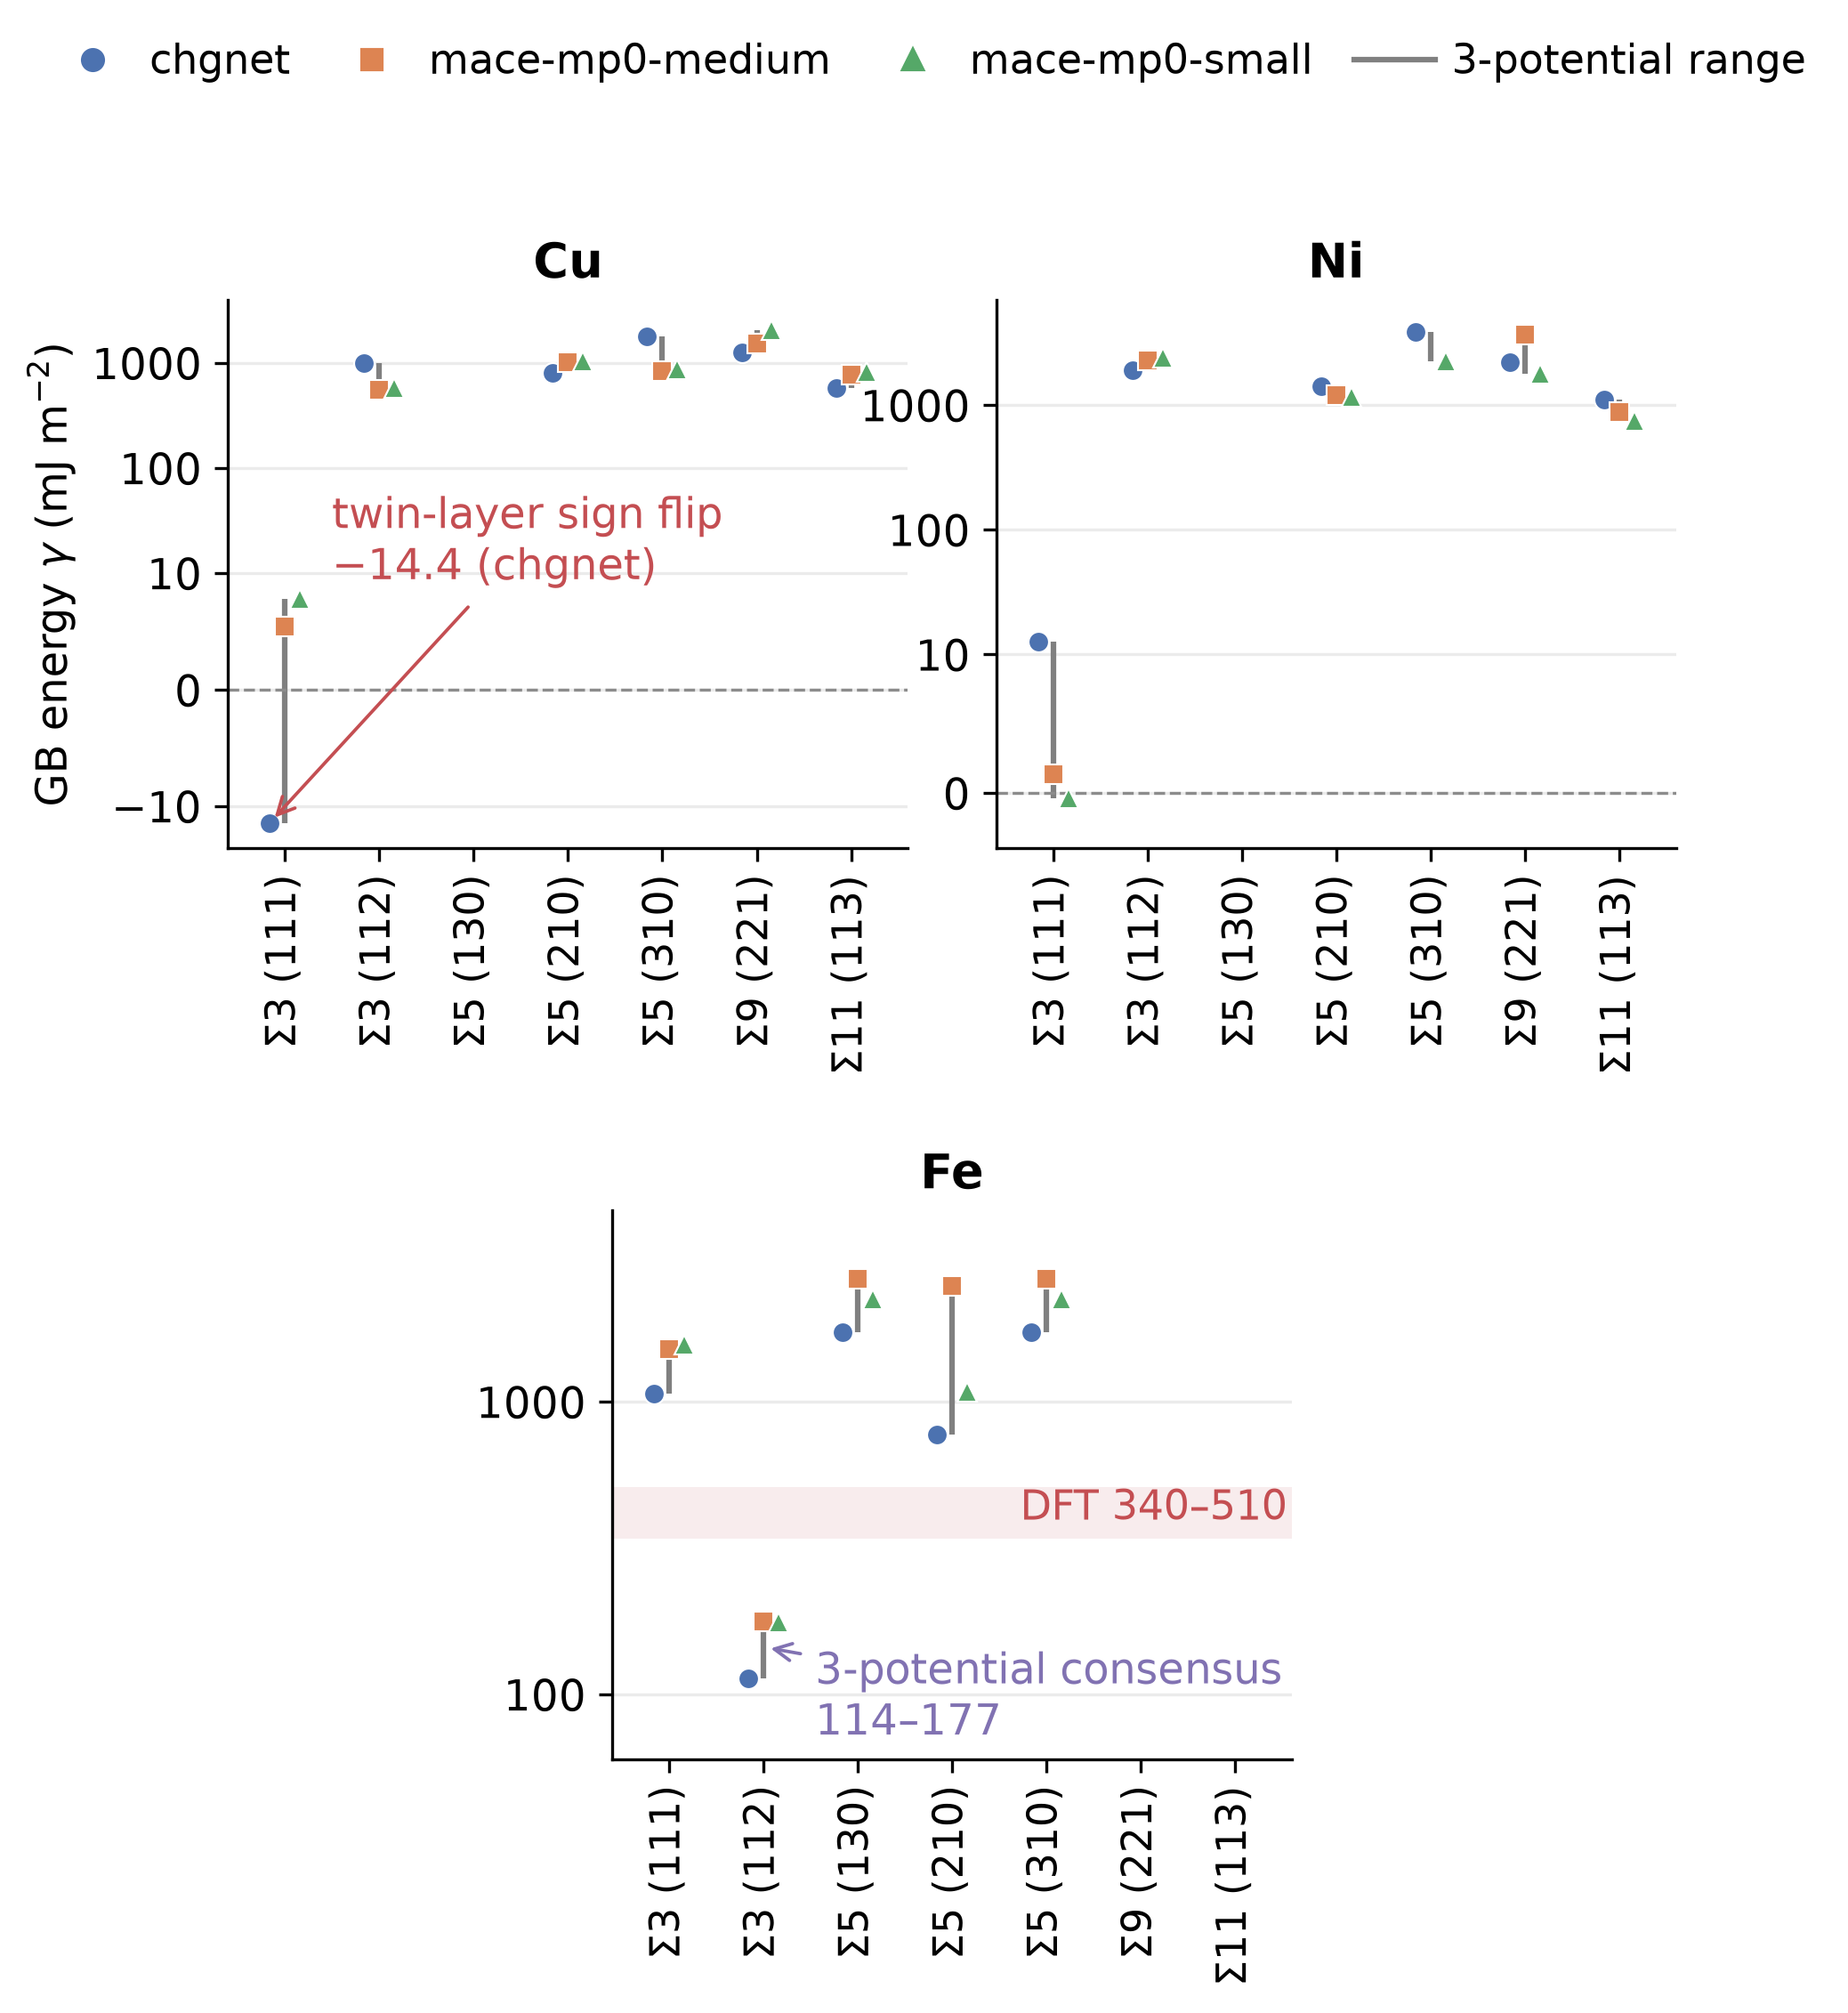
\includegraphics[width=0.9\textwidth]{figures/fig2_energy_spectra.png}
\caption{\textbf{Fig. 1 --- Boundary-energy spectra.} $\gamma$ per GB family for Cu, Ni, Fe under three potentials (symmetric-log scale); grey vertical bars span the three-potential range per family. Annotations: the chgnet Cu $\Sigma$3(111) twin-layer sign flip ($-14.4$ mJ m$^{-2}$) and the three-potential Fe $\Sigma$3(112) consensus (114--177 mJ m$^{-2}$), the tightest inter-potential spread in the library, lying below the shaded ab initio window (340--510 [15]).}
\end{figure}

\begin{figure}[p!]
\centering
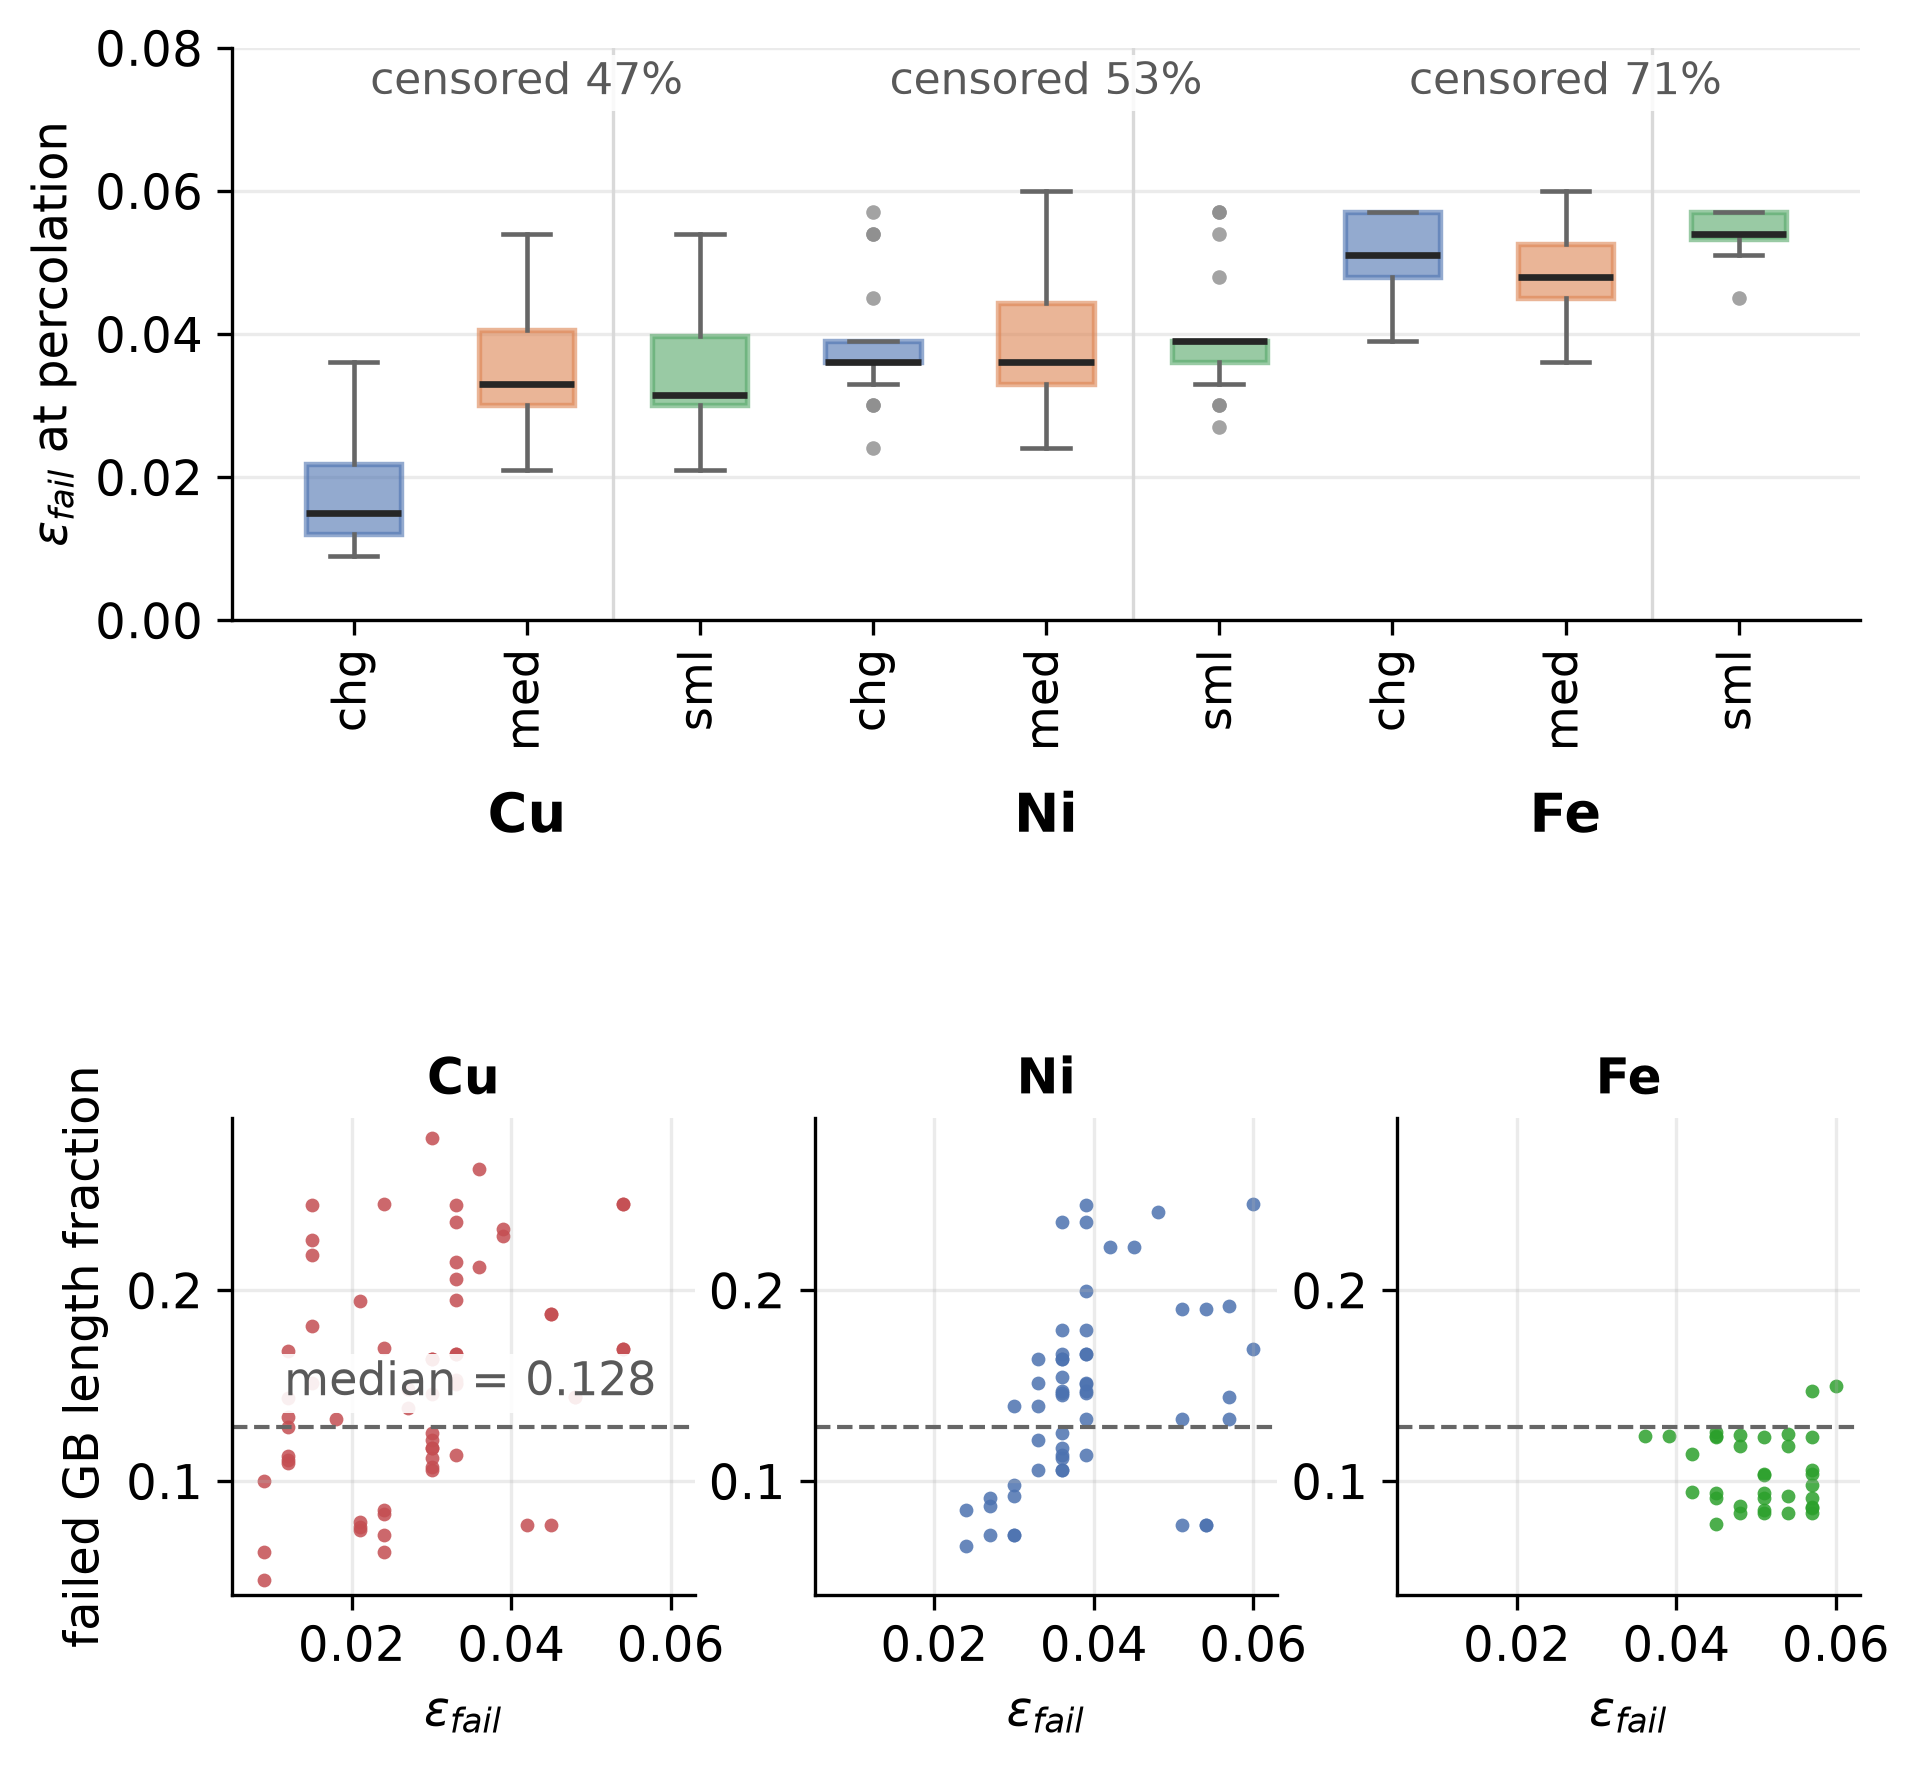
\includegraphics[width=0.9\textwidth]{figures/fig4_labels.png}
\caption{\textbf{Fig. 2 --- Failure labels.} Top: $\varepsilon_{\mathrm{fail}}$ at percolation per potential within each metal (box plots; censored fractions annotated; 155/360 percolated). Bottom: failed GB length fraction versus $\varepsilon_{\mathrm{fail}}$ for percolated labels, one panel per metal (median 0.128) --- percolation occurs at partial, not wholesale, failure.}
\end{figure}

\begin{figure}[p!]
\centering
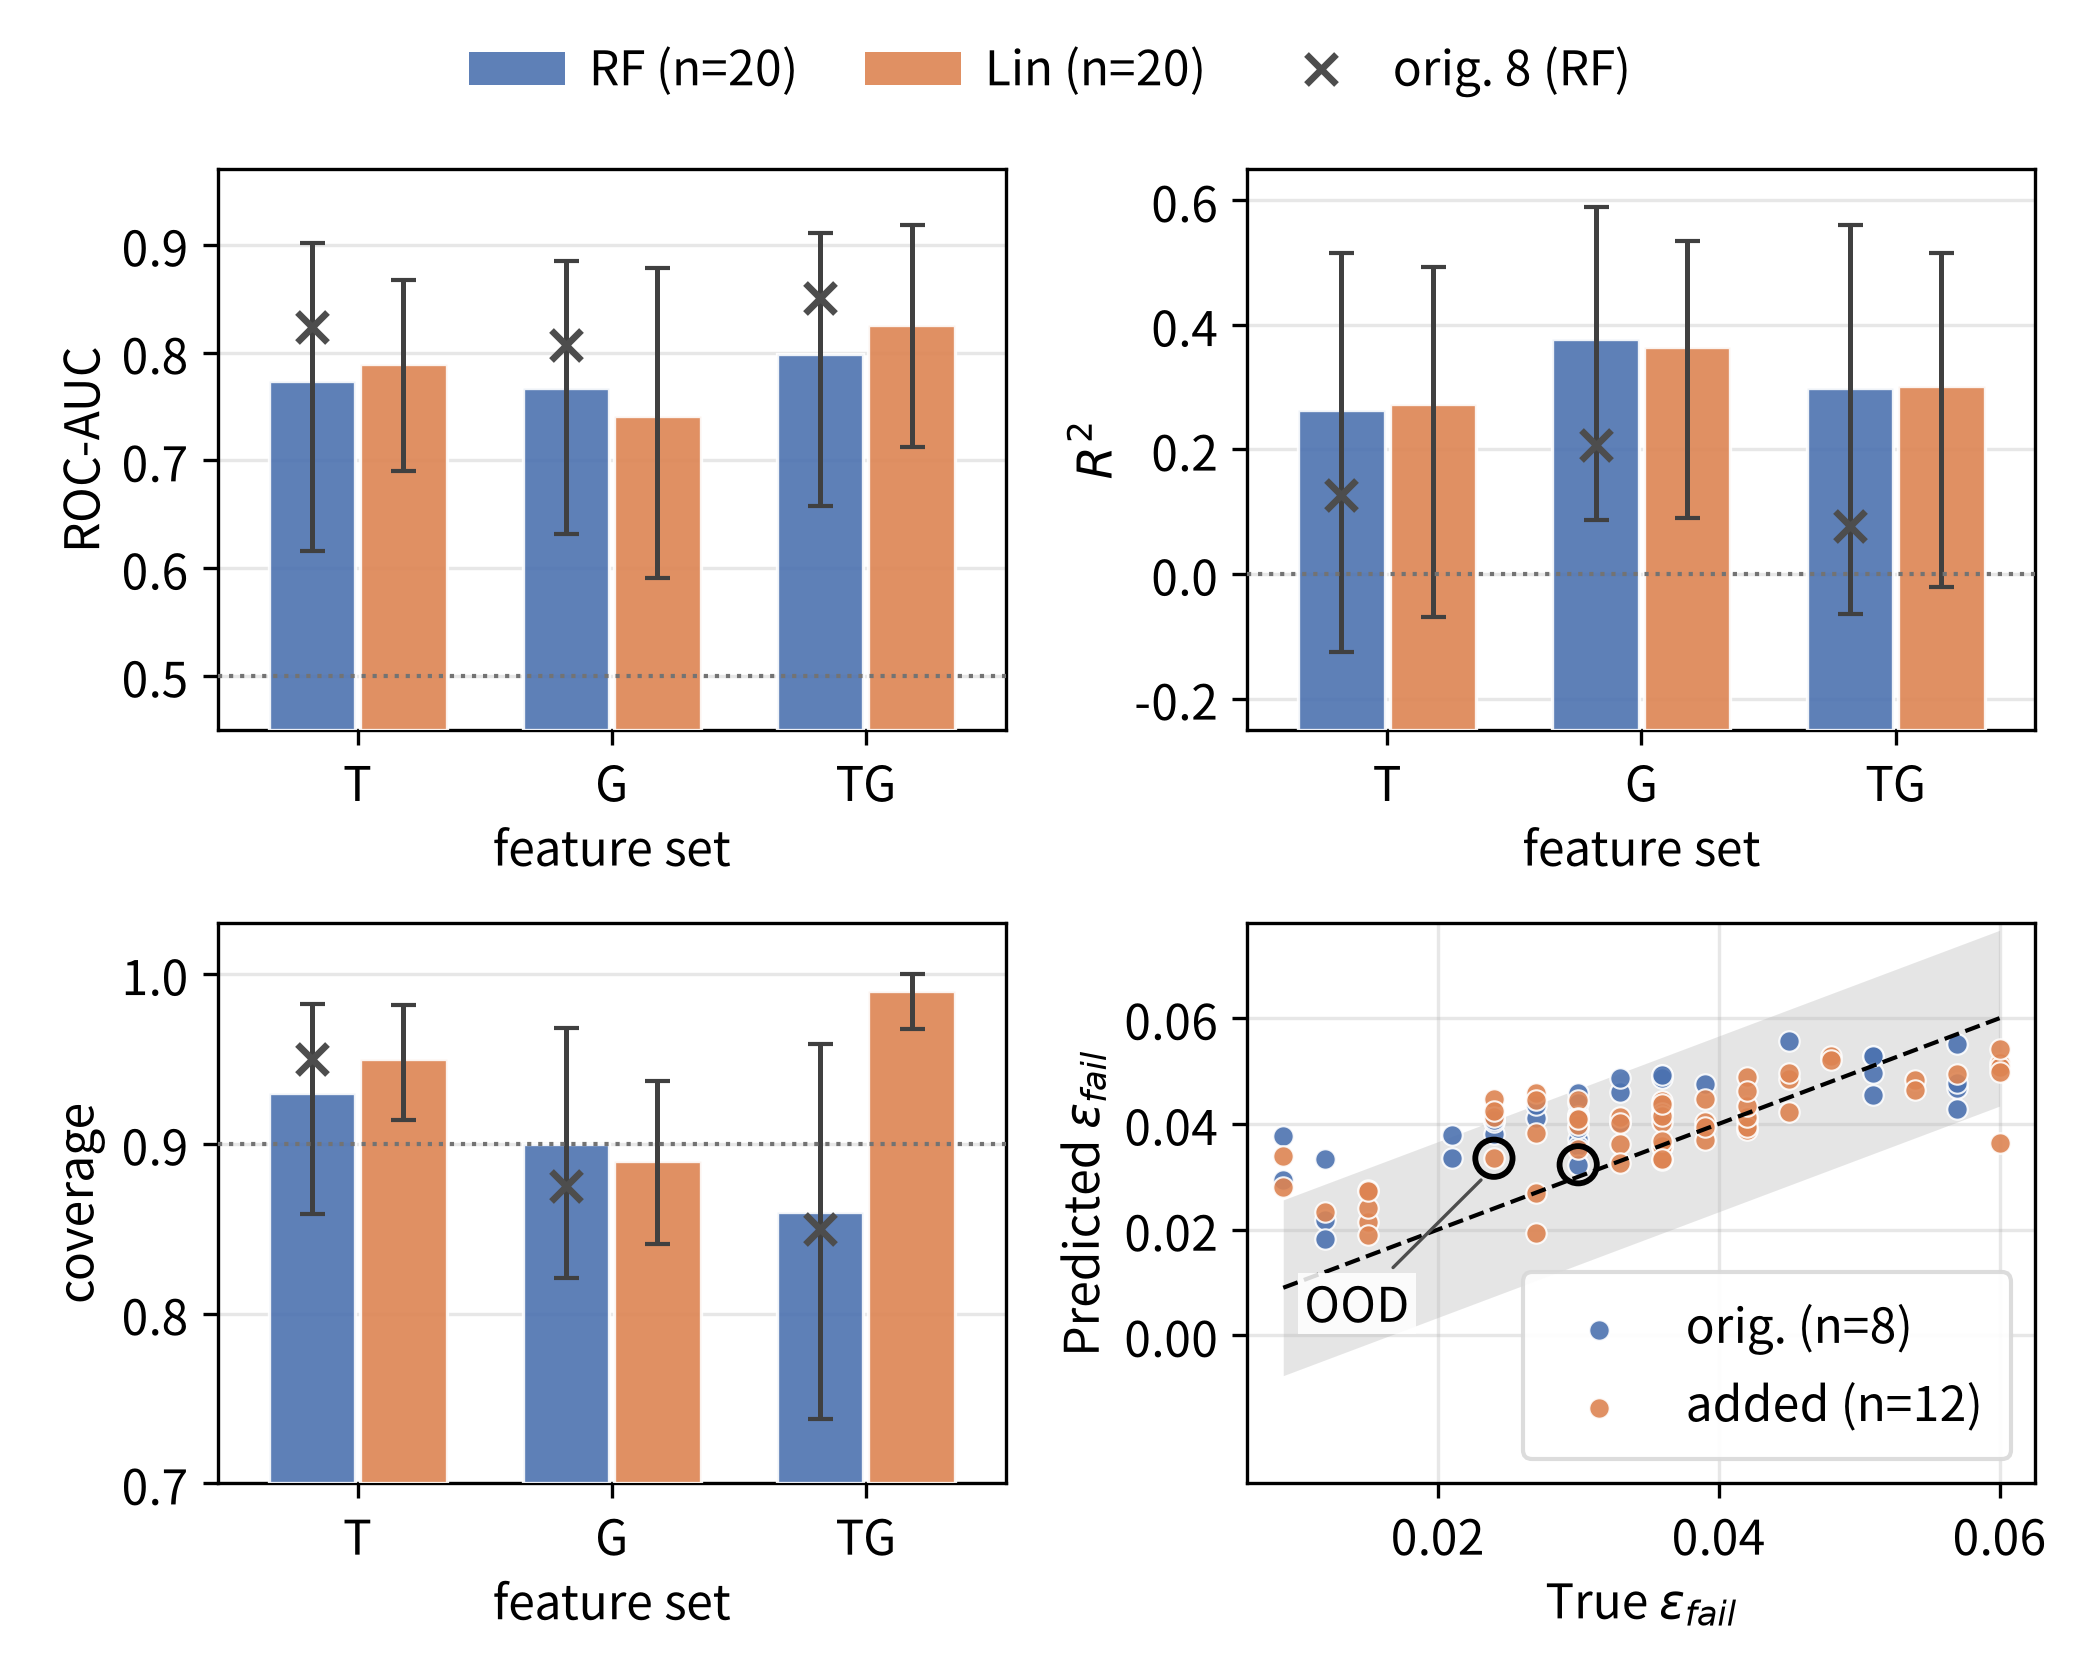
\includegraphics[width=0.9\textwidth]{figures/e4b_blind_ci.png}
\caption{\textbf{Fig. 3 --- Extended blind test with bootstrap confidence intervals (20 microstructures, 180 rows).} Top left/top right/bottom left: blind ROC-AUC, \textit{R}$^{2}$ and conformal coverage for T/G/TG $\times$ RF/linear on the full twenty-microstructure blind set, as grouped bar charts of the point estimate with 95\% microstructure-group bootstrap error bars ($B$ = 2000); grey crosses mark the original eight-microstructure point estimates, dashed lines mark chance (0.5), zero-skill (\textit{R}$^{2}$ = 0) and nominal coverage (0.90). Bottom right: per-row blind $\varepsilon_{\mathrm{fail}}$ predictions (TG-RF, observed coverage 0.860), coloured by original eight versus the twelve microstructures added after the model was frozen; the shaded band is the 90\% conformal interval about the identity line, open black circles mark the two out-of-domain rows among the 100 regression rows.}
\end{figure}

\begin{figure}[p!]
\centering
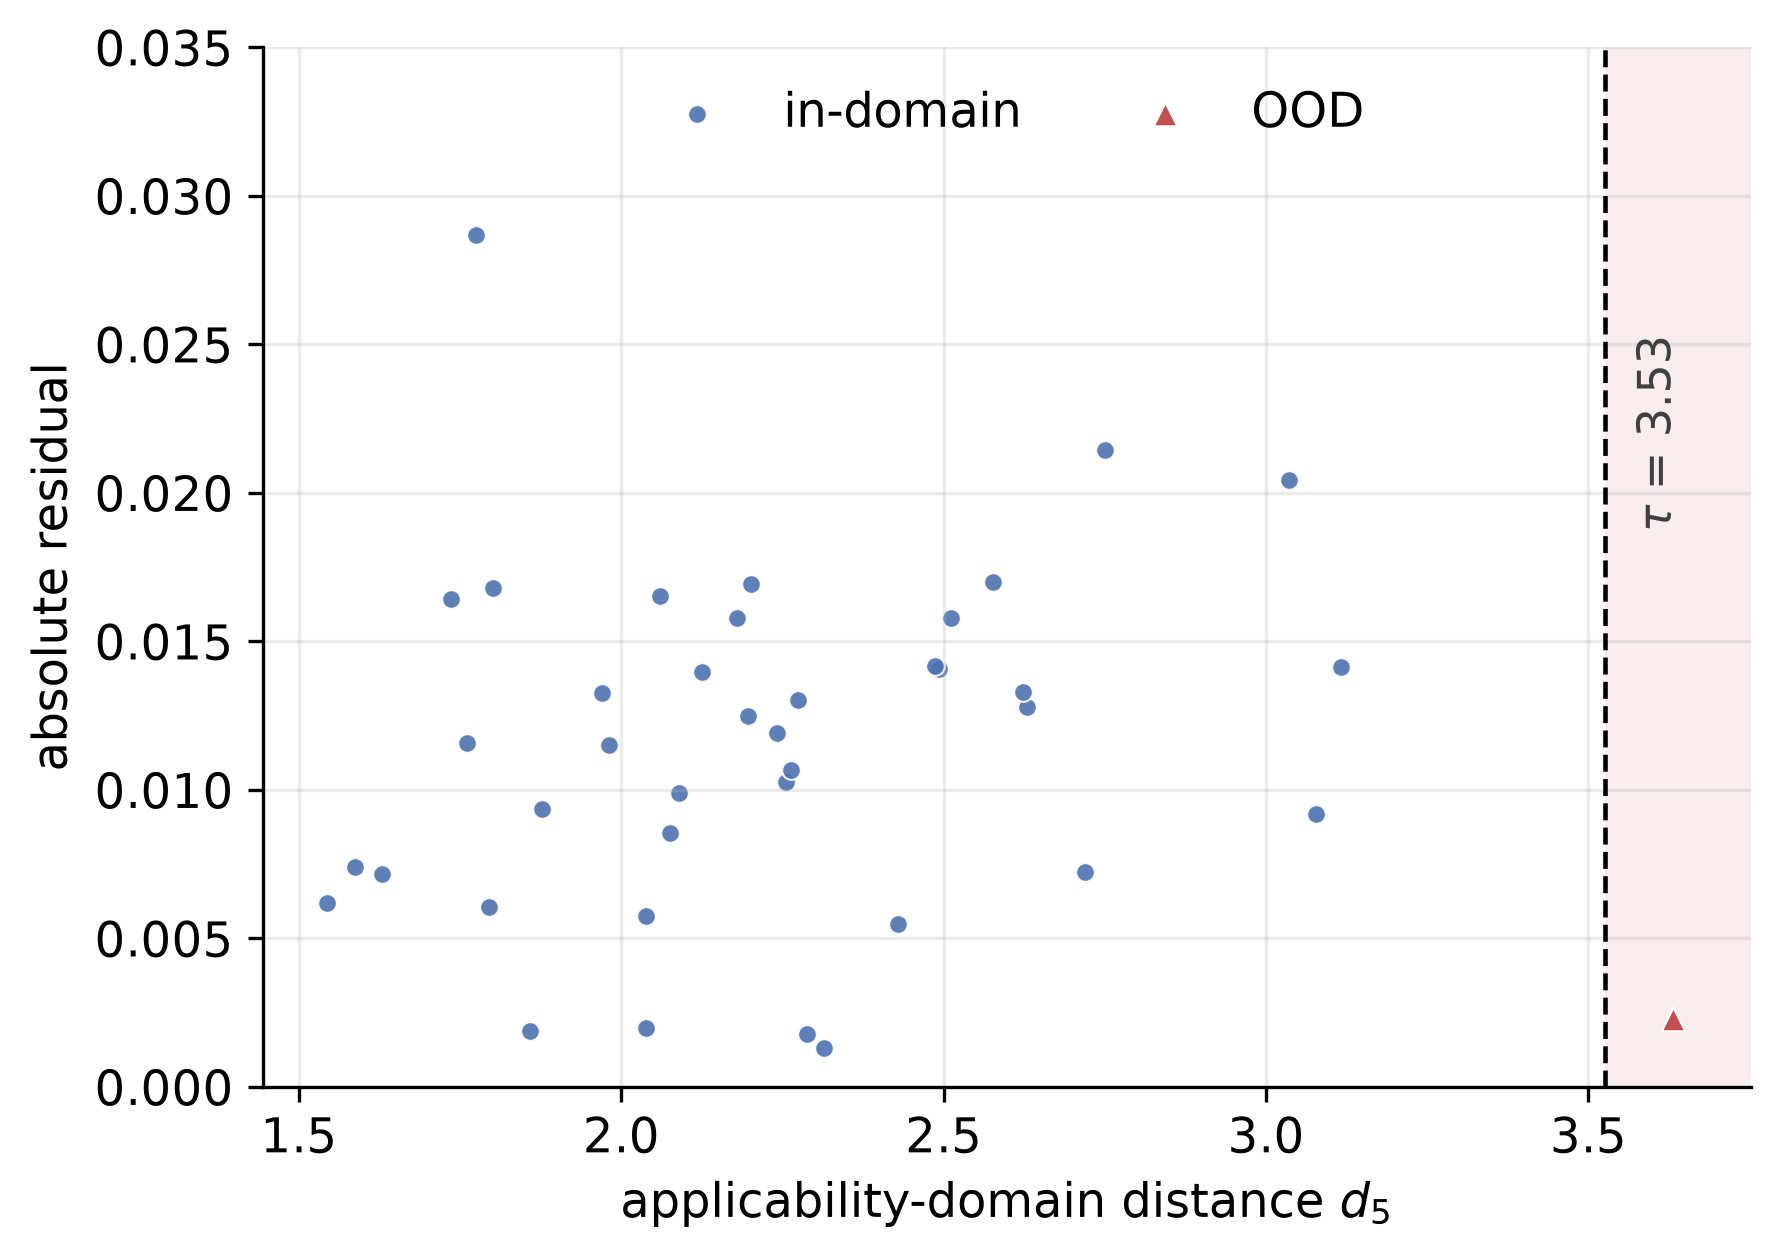
\includegraphics[width=0.9\textwidth]{figures/fig6_domain.png}
\caption{\textbf{Fig. 4 --- Applicability domain.} Absolute residual versus 5-nearest-neighbour domain distance $d_5$ for blind regression rows of the original eight microstructures (TG-RF); dashed line at $\tau$ = 3.53 (95th percentile of calibration distance) bounds the shaded out-of-domain region. OOD rows marked.}
\end{figure}

\begin{figure}[p!]
\centering
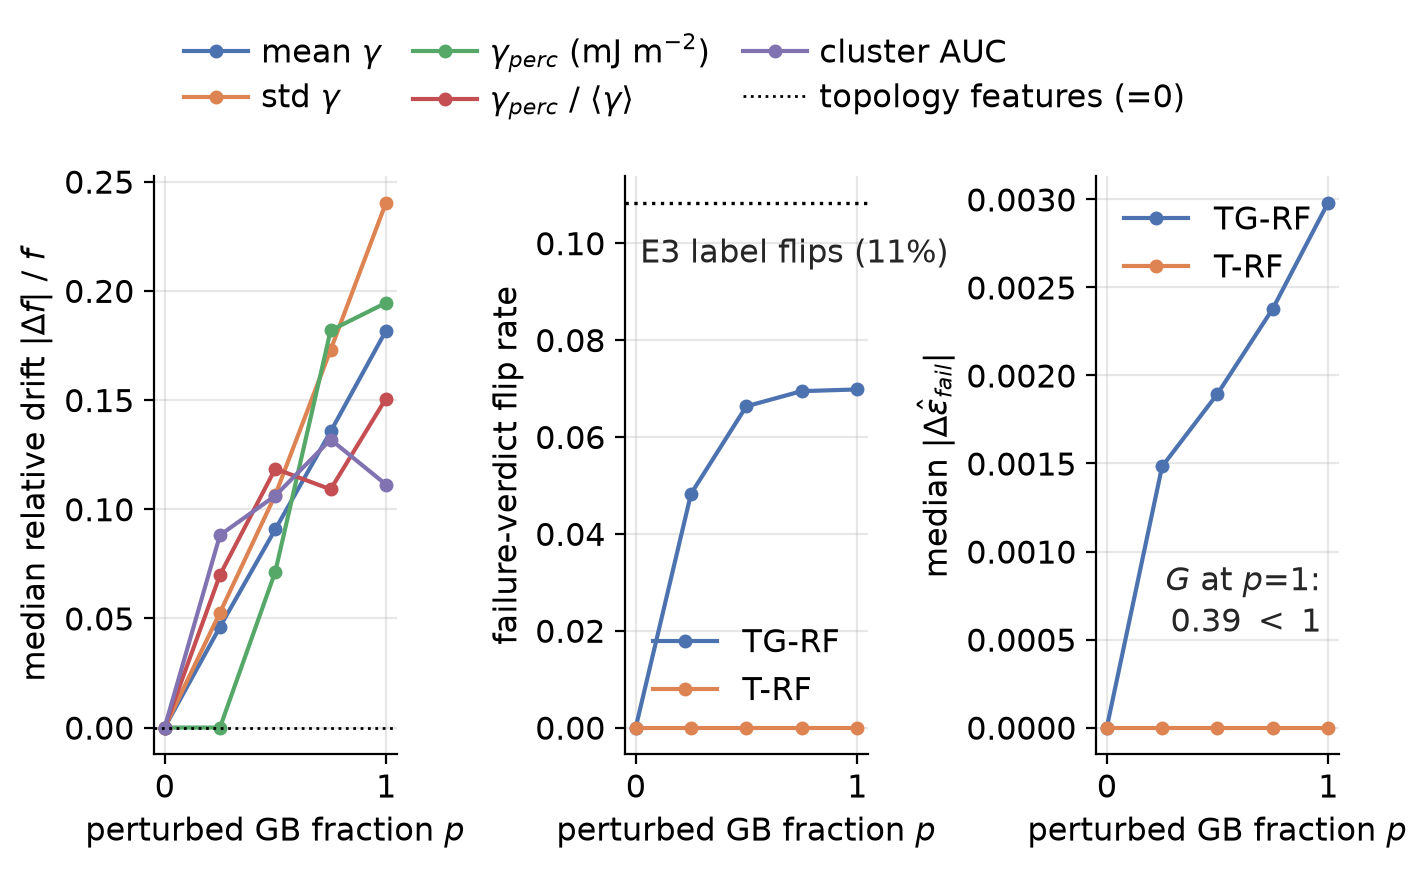
\includegraphics[width=0.9\textwidth]{figures/fig7_propagation.png}
\caption{\textbf{Fig. 5 --- Error propagation.} Left: median relative feature drift versus perturbed fraction \textit{p} (topology features exactly zero). Centre: binary verdict flip rate versus \textit{p}, with the label-side cross-potential instability (11\%) as anchor. Right: regression drift versus \textit{p} with propagation gain $G$ annotated (all $<$ 1).}
\end{figure}

\end{document}
